\section{Classification Examples and Exercises}
\textcolor{commentGreen}{*** WIP ***}

\subsection{Illustrated Example 1: A surface contact has been detected can you narrow down its class or type?}
\large Difficulty Rating \includegraphics{../img/actuals/Stars/"1 Star.jpg"}

\subsubsection{MNW In Game Tools}

A surface contact has been identified on broadband. Trackers are assigned for the LAB, WAA and the TB34 “Fatline” towed array. Listening to the sound from the LAB you hear:

\begin{compactenum}
    \item A distinct fast “swooshing” sound which you think maybe cavitation noise
    \item A faster underlying “tchouc tchouc tchouc” sound which you think is propellor blade noise
    \item You do not hear sounds characteristic of a diesel engine
    \item You do hear a prominent high pitch whine which sounds like a turbine or a high speed gear mesh
\end{compactenum}


Your initial conclusion is that this is a modern turbine powered ship cruising at a medium speed (15 - 25 kts) and that it is probably a warship. You base your provisional conclusions on the following tables from your personal notebook and the knowledge that most civilian ships are not turbine driven.

Civilian

\begin{tabularx}{\linewidth}{l l l X}
    \toprule
    \textbf{Speed Category} & \textbf{Knots} & \textbf{km/h} & \textbf{Typical Examples}\\
    \midrule
    \rowcolor[gray]{.9}Slow & Under 12 kn & Under 22 km/h & Large tankers, heavily loaded bulk carriers \\
    Medium & 12 - 20 kn & 22 - 37 km/h & Most cargo ships, ferries, many merchant vessels \\
    \rowcolor[gray]{.9}Fast & 20 - 30 kn & 37 - 56 km/h  & Cruise ships, fast ferries, some naval vessels\\
    Very fast & 30+ kn & 56+ km/h & Destroyers, patrol boats, high-speed ferries\\
    \bottomrule
\end{tabularx}

Warship

\begin{tabularx}{\linewidth}{l l l X}
\toprule
\textbf{Speed Category} & \textbf{Knots} & \textbf{km/h} & \textbf{Typical Examples}\\
\midrule
\rowcolor[gray]{.9}Slow & Under 15 kn & Under 28 km/h & Economic cruising, patrol, or fuel-saving transit \\
Medium & 15 - 25 kn & 28 - 46 km/h & Normal operating speed for most missions \\
\rowcolor[gray]{.9}Fast & 25 - 35 kn & 46 - 65 km/h  & High-speed transit, tactical maneuvers\\
Very fast & 35+ kn & 65+ km/h & Fast attack craft, some hydrofoils, exceptional warships\\
\bottomrule
\end{tabularx}

Using the sound output feature of the sonar suite you find it is possible to count the more prominent “swooshing” sound. You do this over 60 seconds several times then take an average. By doing this you establish that there are an average of 130 beats per minute which is about 2.1 Hz (130 / 60). Unfortunately you can't do the same for the higher frequency blade rate as there is no facility to slow the sound down in game at this time.

Top Tip: Counting sounds like this can be made much easier by using a beat tap counter which will automatically give you the count / beats per minute. Some will even listen to the sound and give you a count. There are several available free for iPad / iPhone and Android

In MNW you switch to narrowband and attach the TB34. You start at a wide window of frequencies (0 - 3600 Hz) which produces the following display (Figure 16).

You immediately recognise a fairly strong tonal at 3 kHz (3000 Hz) which you think is the high pitched whine which you attribute to the turbine or possibly the reduction gear. You also spot a strong diffuse band centred around 261 HZ (150 - 400 Hz) and another less prominent band between 1050 and 1350 Hz.

At this scale it is not possible to see any other tonals so you select a drilled in view (Figure 17). At this frequency range it is possible to see another faint tonal around 33 Hz. This is quite difficult to spot and requires high input and gain settings which washes out most of the screen so details within the broader noise bands are lost. At this stage you do not know what is causing the 33 Hz tonal so you carefully note it before moving on to a DEMON analysis in an effort to gain some insight into the ship’s speed.

DEMON can provide information about the shaft rate (SR) and the blade count (BC). Sometimes it is possible to identify the number of propeller shafts (Figure 18). Our system shows a strong tonal at 2.2 Hz (Note in the picture the cursor is offset) which is hypothesised to be the shaft fundamental.

\begin{figure}[ht]
	\centering
	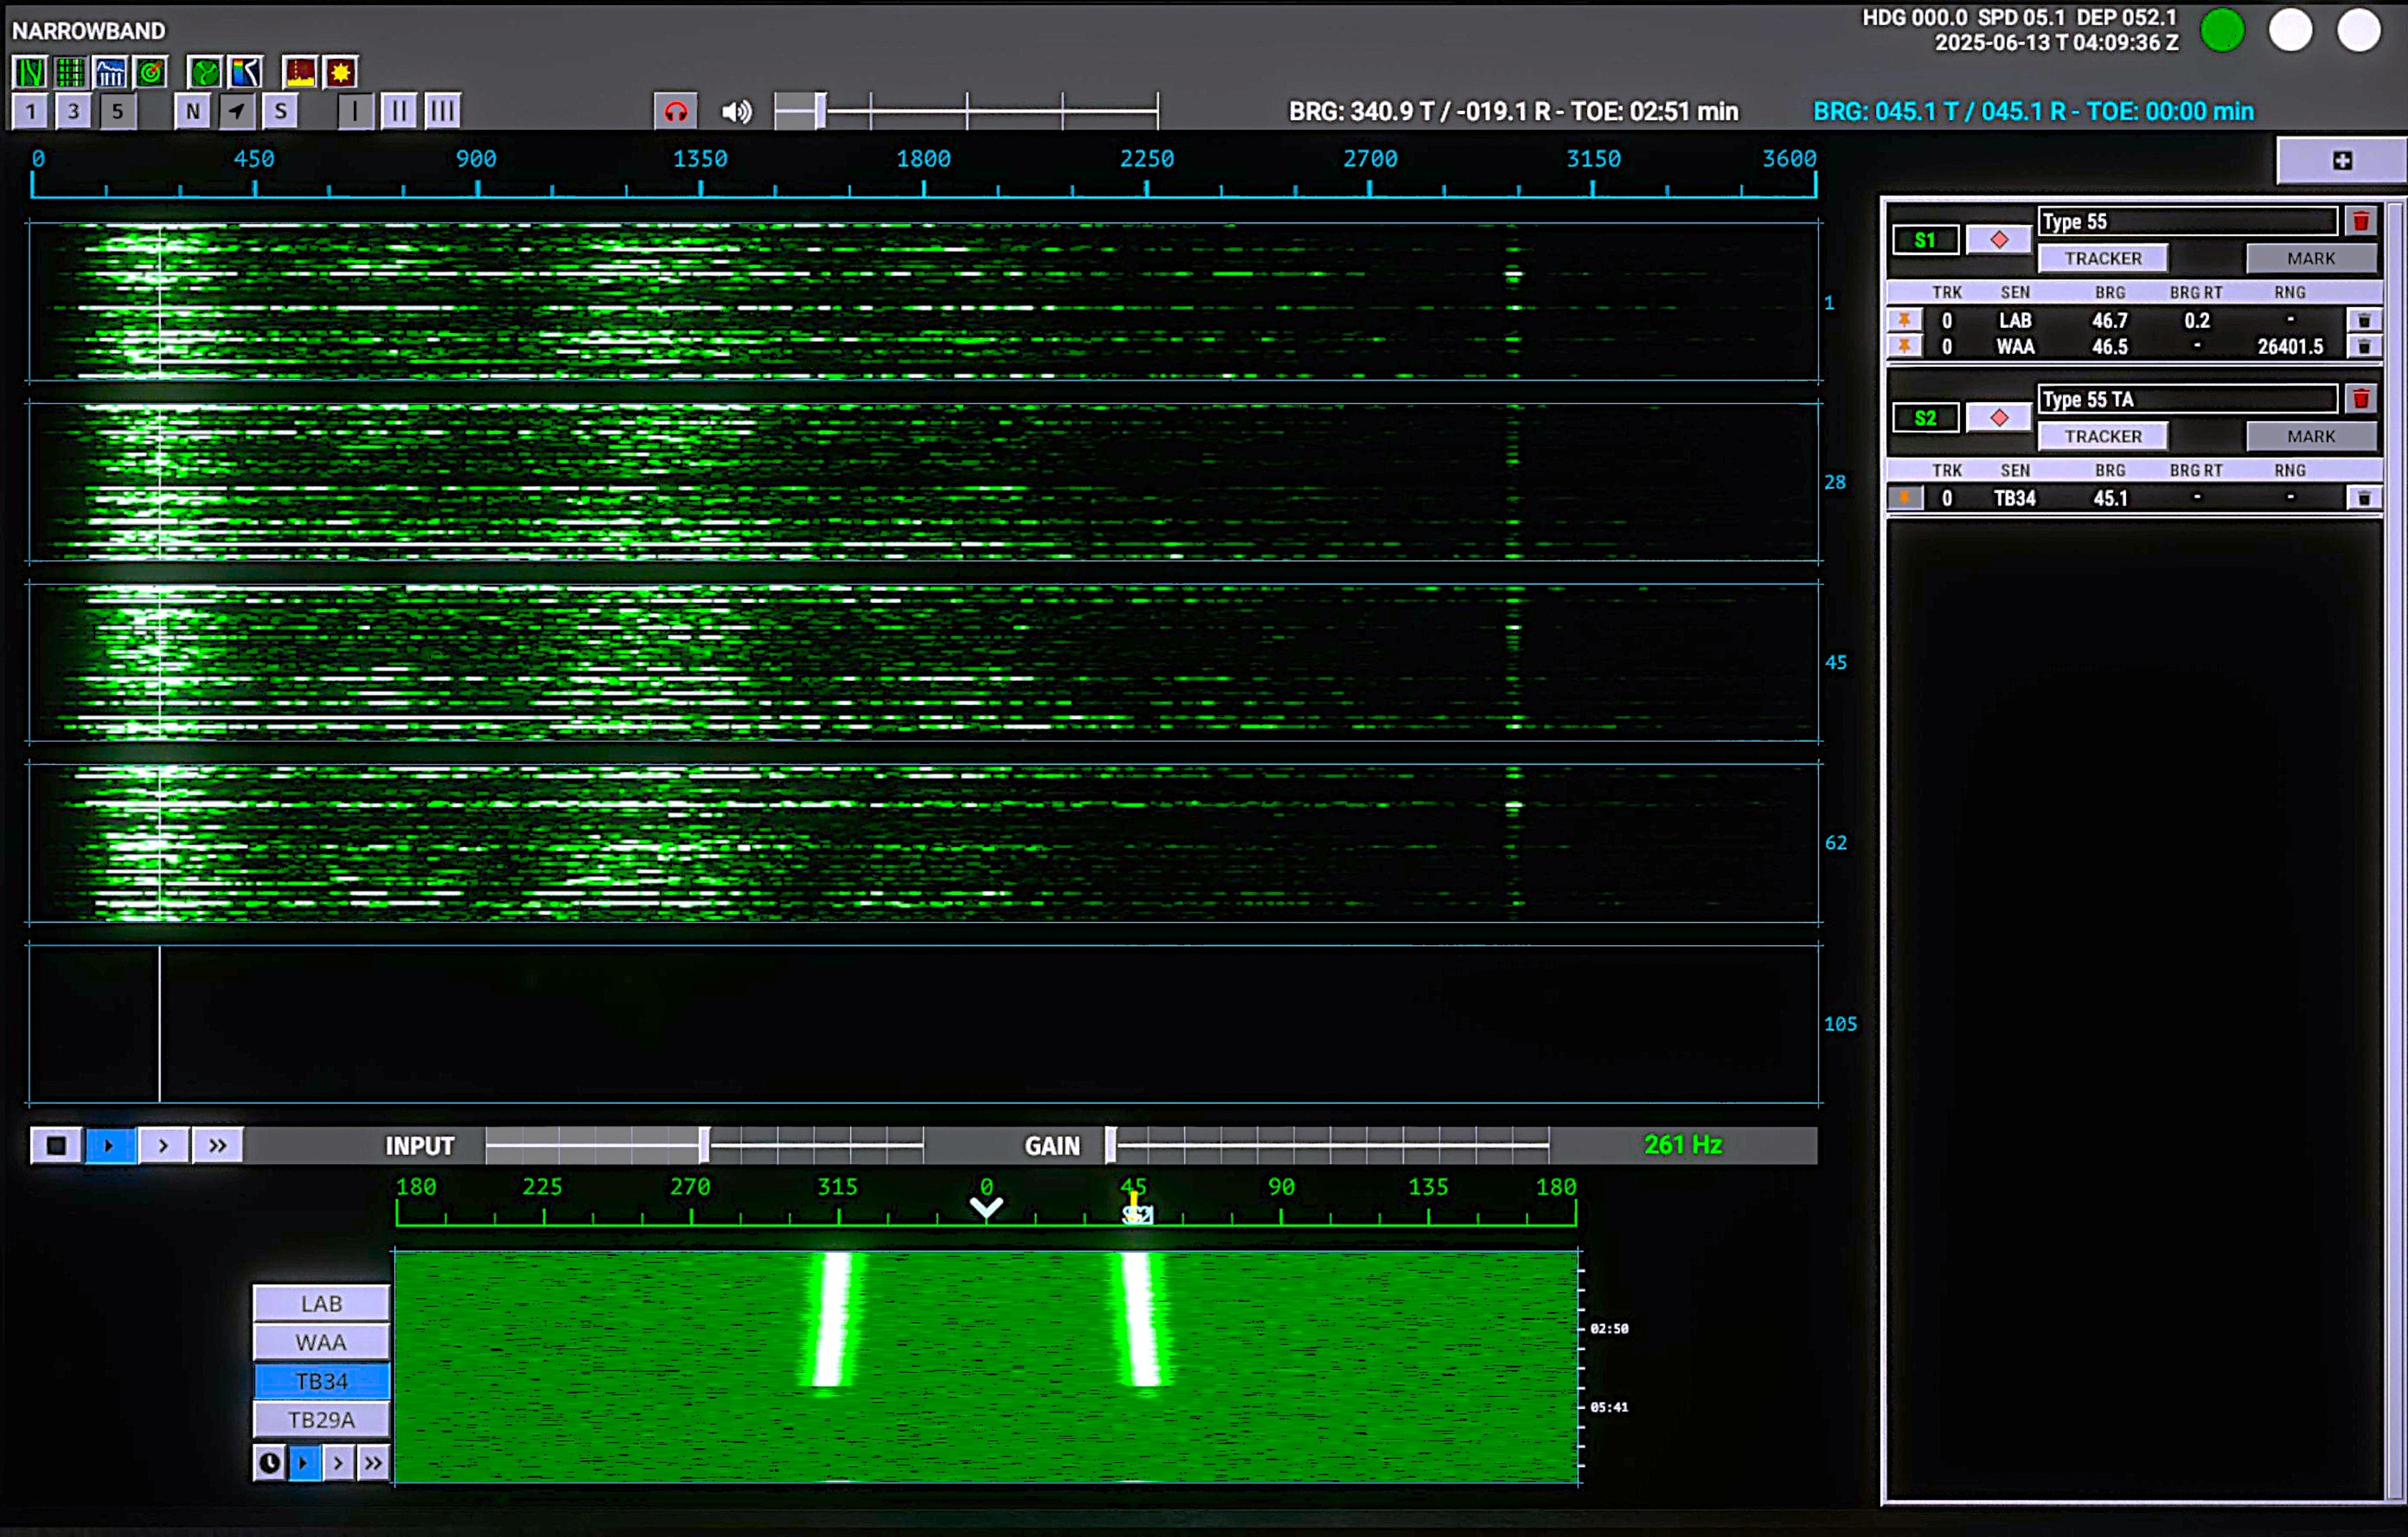
\includegraphics[width=310px]{../img/actuals/Type55_01a.pdf}
	\caption{Narrowband 0 - 3600 Hz}
\end{figure}

\begin{figure}[ht]
	\centering
	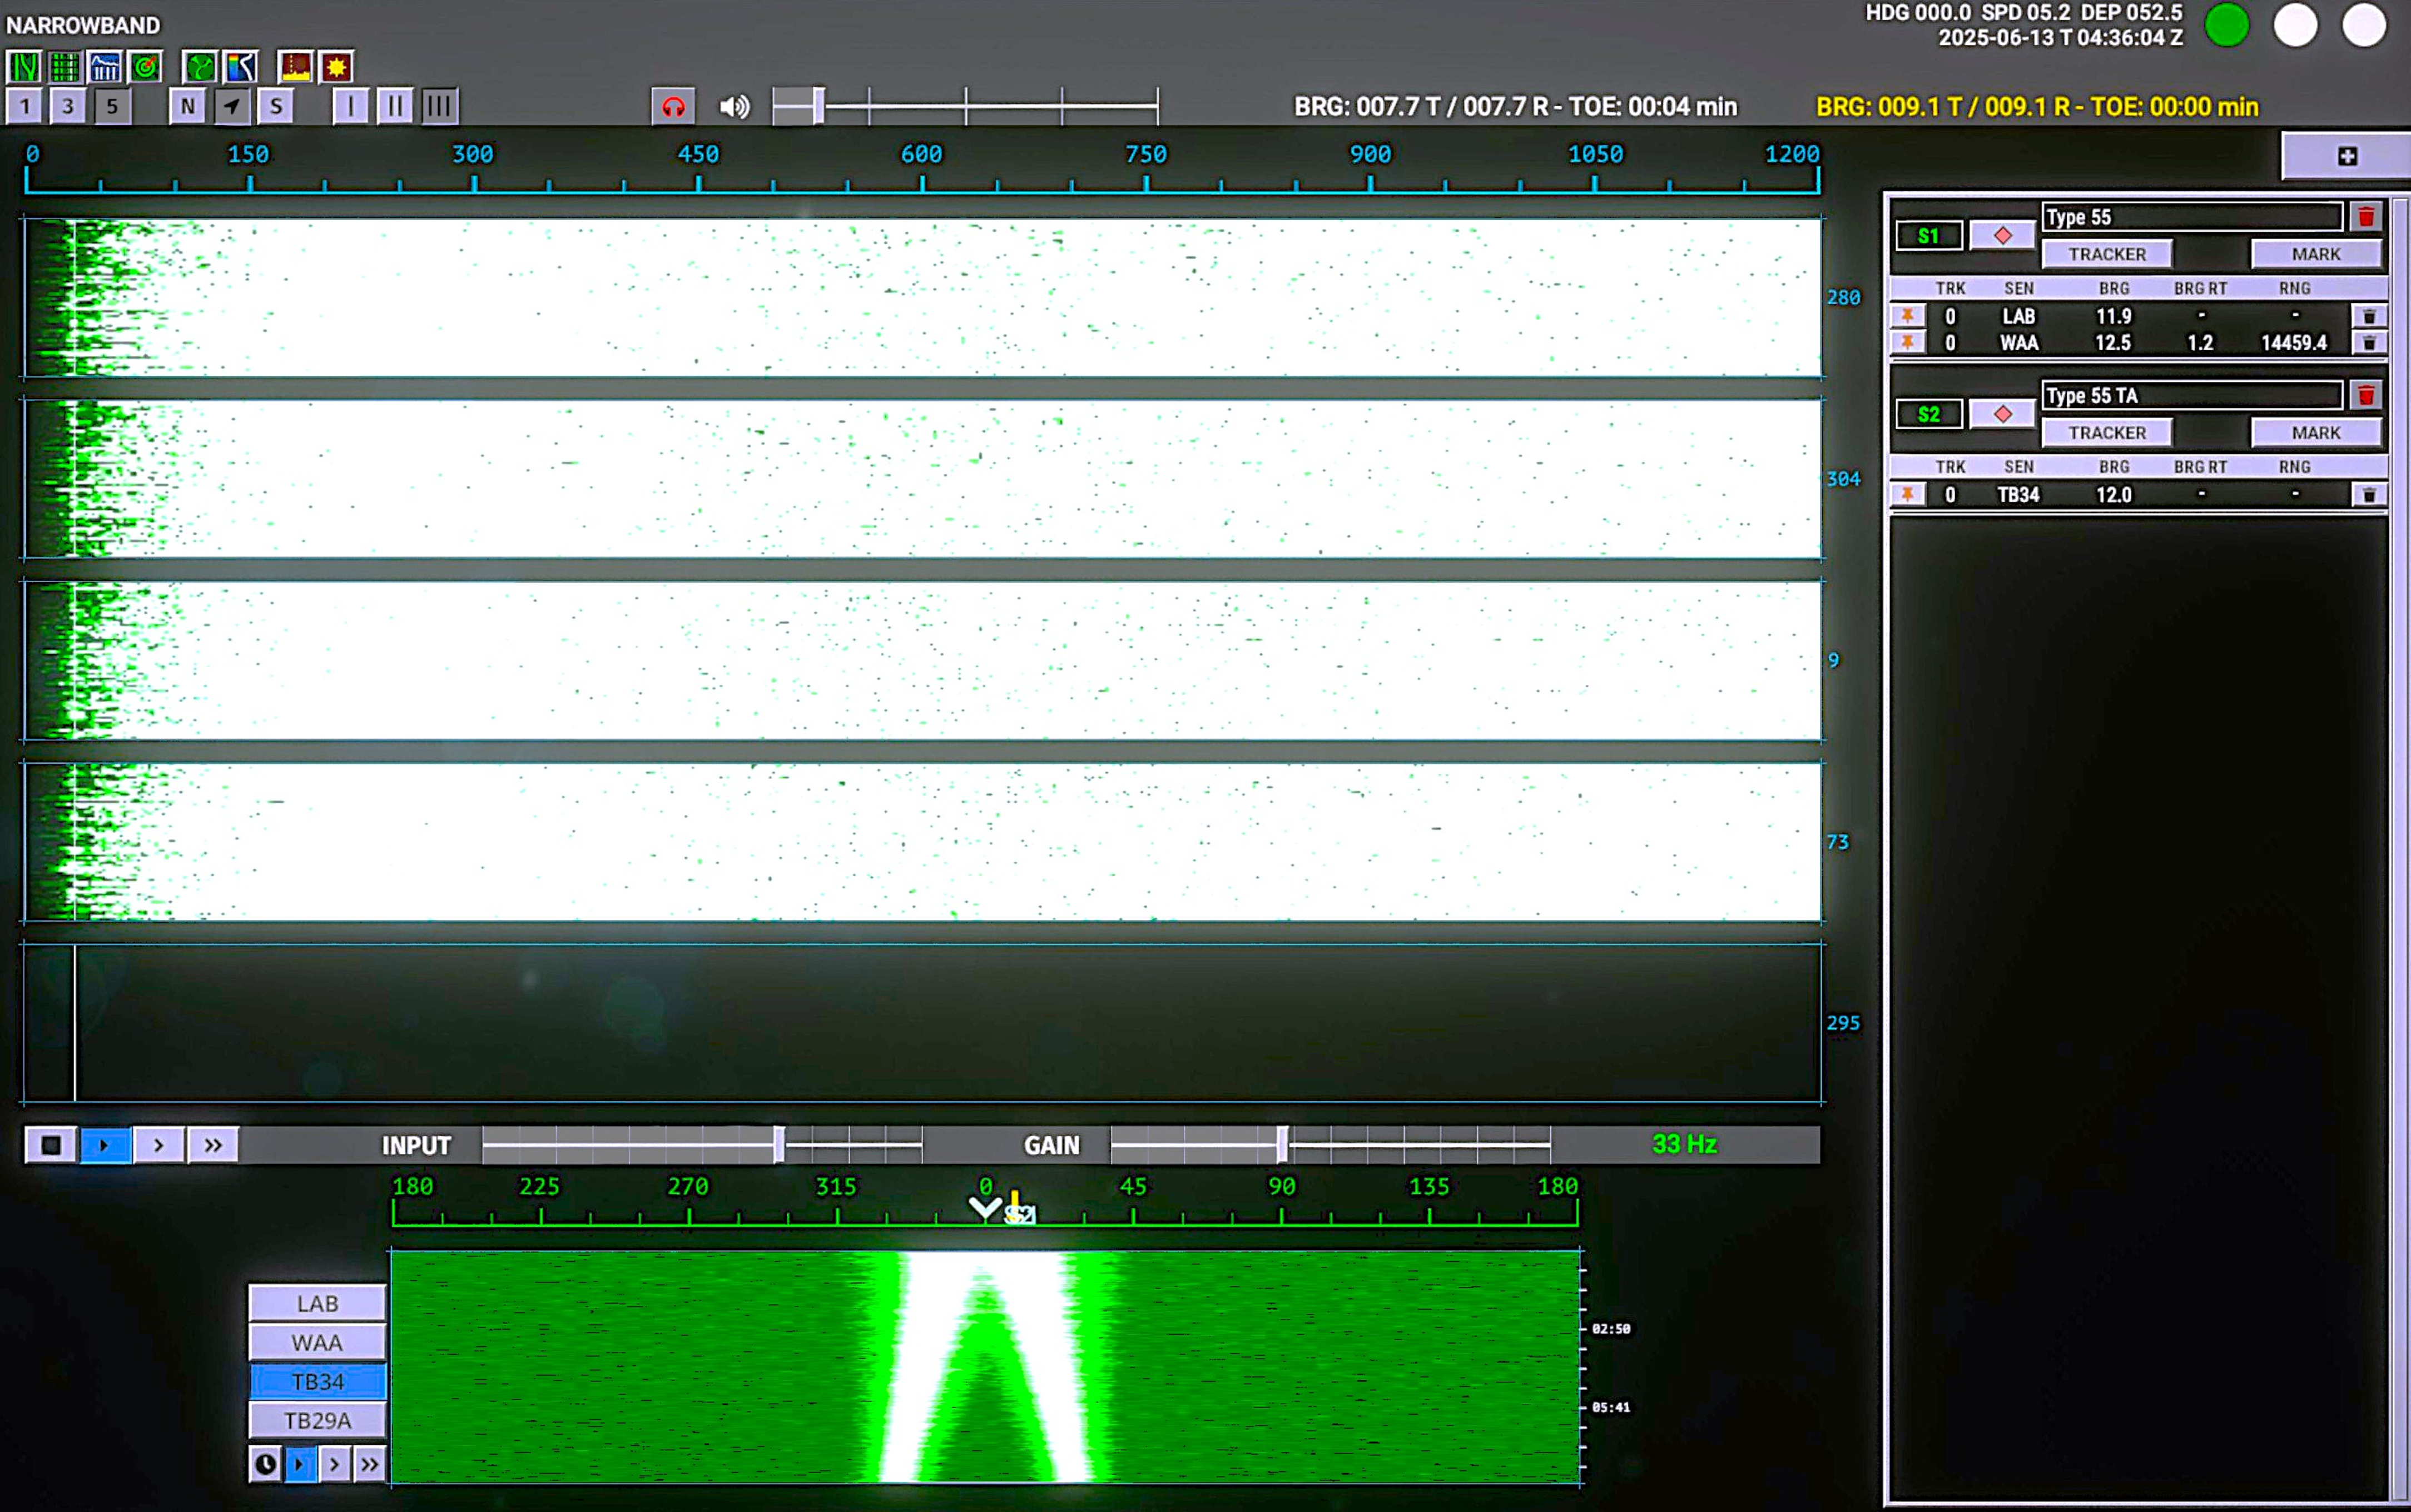
\includegraphics[width=310px]{../img/actuals/Type55_01b.pdf}
	\caption{Narrowband 0 - 1200 Hz - a faint 33Hz tonal}
\end{figure}

\begin{figure}[H]
	\centering
	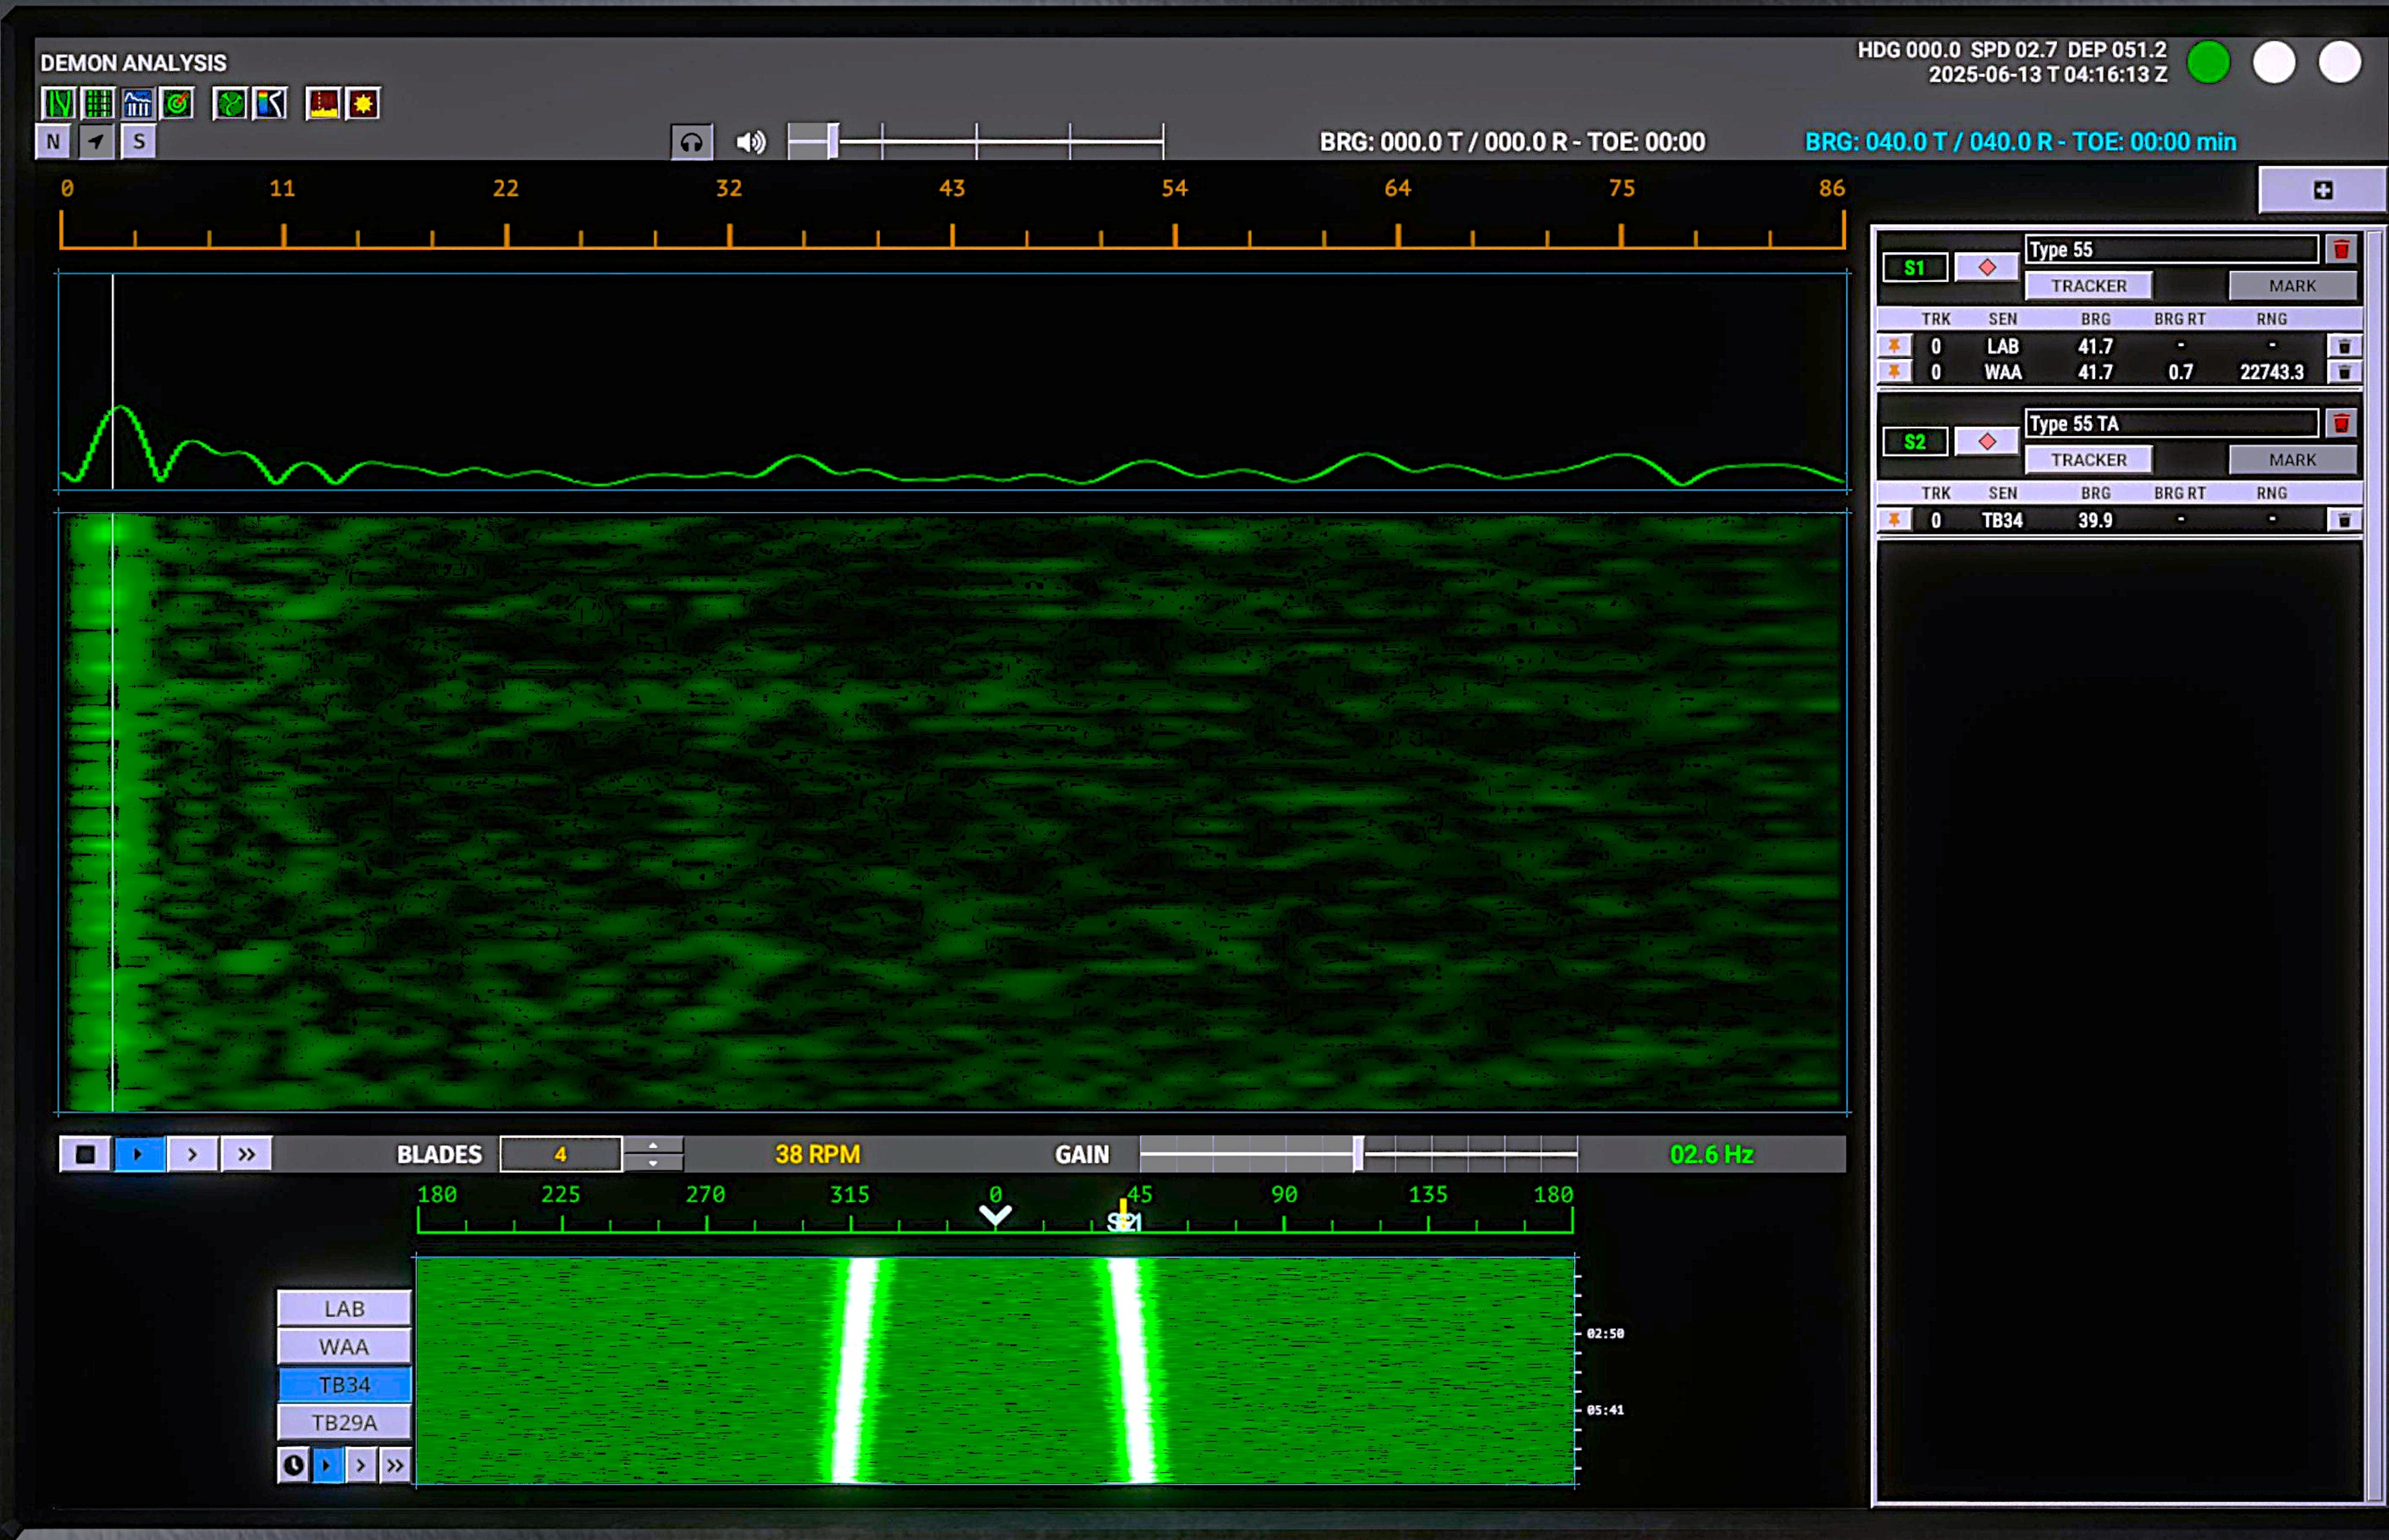
\includegraphics[width=310px]{../img/actuals/Type55_02.pdf}
	\caption{DEMON Display}
\end{figure}

It is difficult to get the exact frequency because the tonal is quite smeared as if there were two lines on top of each other slightly offset. If that were the case it would suggest this vessel has at least two shafts. The rotation frequency of 2.2 Hz gives a shaft rotation speed of 132 RPM ($2.2 \times 60$).

The DEMON waterfall is not providing any clear indication of the number of propeller blades, however the smooth line plot above does show some slight indication of blades. Including the shaft it is just possible to suggest 5 humps and then a series of what could be harmonics further up. This could be indicative of a five bladed propeller which, if this is true would give a blade rate of 11 Hz ($5 \times 2.2$) or 660 RPM ($11 \times 60$). However, the data is speculative and definitely requires a more detailed analysis.

\subsubsection{MACS Tools}

In order to improve your analysis and refine your hypothesis you decide to utilise the advanced tools available in MACS.

Your first step is to capture a recording of the sound of the contact. How to do this depends on your PC sound configuration but most often this will be a simple loopback arrangement (See Section 3). Capture a recording by clicking the record button on the top toolbar. The recording should be long enough to capture any periodic variation in the sound, 2 minutes should be plenty although longer recordings may be necessary if you are monitoring changes of speed or direction. As soon as you stop the recording it will appear in the recordings panel on the lower right of the application. It is highly recommended that you change the generated name to one that is more user friendly. Do this by double clicking the recording and renaming it. Once you have your recording you can analyse the sound in a more structured way without having to deal with real time issues.

As for the in game tools your first review should be using your ears and your experience. We can tell from the recording that:

\begin{compactenum}
    \item No diesel firing.
    \item Distinct slower “swooshing” sound.
    \item Underlying faster “blade” sound.
    \item High pitched whine at 3 kHz possibly turbine or gear mesh.
\end{compactenum}


You first focus on the 3 kHz tonal which you believe is responsible for the high pitched whine which you suggest is either the turbine or the reduction gear mesh frequency. By setting the bandpass frequency to 0 - 2500Hz the sound is eliminated from the playback strengthening the hypothesis.

Next assess the distinctive audible regular “swooshing” sound and the faster chopping sound. Using a beat counter the louder sound is found to be 134 BPM. You propose that the sound is made by cavitation and can be used to estimate the shaft RPM. 134 RPM is 2.2 Hz. When we come to look at the LOFARgram we will look out for the shaft fundamental at that value.

Counting the Blade Rate is more difficult because it is too fast. Using MACS we have the option to slow the playback, a feature MNW does not have at this point. Slowing the playback speed to 0.25 it is possible to count each blade passing. For this exercise several counts over 30 seconds were conducted and then averaged.

Blade RPM playback at 0.25 speed over 30s averaged: $82 \times 2 \times 4$ ( $\times 2$ because 30s $\rightarrow$ 1 minute and $\times 4$ because 0.25 speed) = 656 RPM or 11 Hz

Blades: $654 \div 134 = 4.9$ (5 Blades) It is always likely that the numbers will not be exact as the sound path from source to receiver is never as straight forward as theory would suggest. Propellers can be out of balance and modulate shaft and blade sounds. Gears and bearings wear unevenly. Ships can change speed and direction introducing doppler effects which can distort or enhance frequencies. Bear in mind these “confounders”, you should expect measures never to be exact. You will use your experience to judge whether 4.9 should be 5 when 4.69 is too many deviations to be reliable.

\begin{faintquote}
    Top Tip: Take notes continuously they will become a powerful tool to help you be more effective and efficient at narrowing down target classification
\end{faintquote}

\begin{faintquote}
    It should be clear by now that the process is one of hypothesis forming, testing and falsification. Ultimately you are never going to be 100\% confident in your analysis it is always going to be on the balance of probabilities. Becoming comfortable with working with uncertainty is key to being effective.
\end{faintquote}

\textbf{LOFAR}

Our next step is to look at MACS' equivalent of the MNW's narrowband and DEMON plus some additional tools that have yet to appear in game.

One of the many features of MACS is the ability to tune input and output parameters. This is, at the time of writing, quite limited in game. To get the best results you will need to tweak these parameters so you must understand what they do. Details are discussed in Sections 2 and 5 and Appendix B. Unfortunately it is not possible to give hard and fast guidance as everyone's screens will vary in capability, refresh rates or resolution. For Figure 19 the following settings were used.

\begin{compactenum}
    \item Fmin = 0 Fmax = 5000
    \item Floor = -90 Dyn = 55
    \item Norm = Off
    \item FFT Overlap = Off
    \item FFT = 131072
\end{compactenum}

Note: This level of detail is very slow to plot however this is realistic. It is possible to speed things up by reducing the FFT or increasing the overlap setting at the cost of reducing detail.

\begin{figure}[ht]
	\centering
	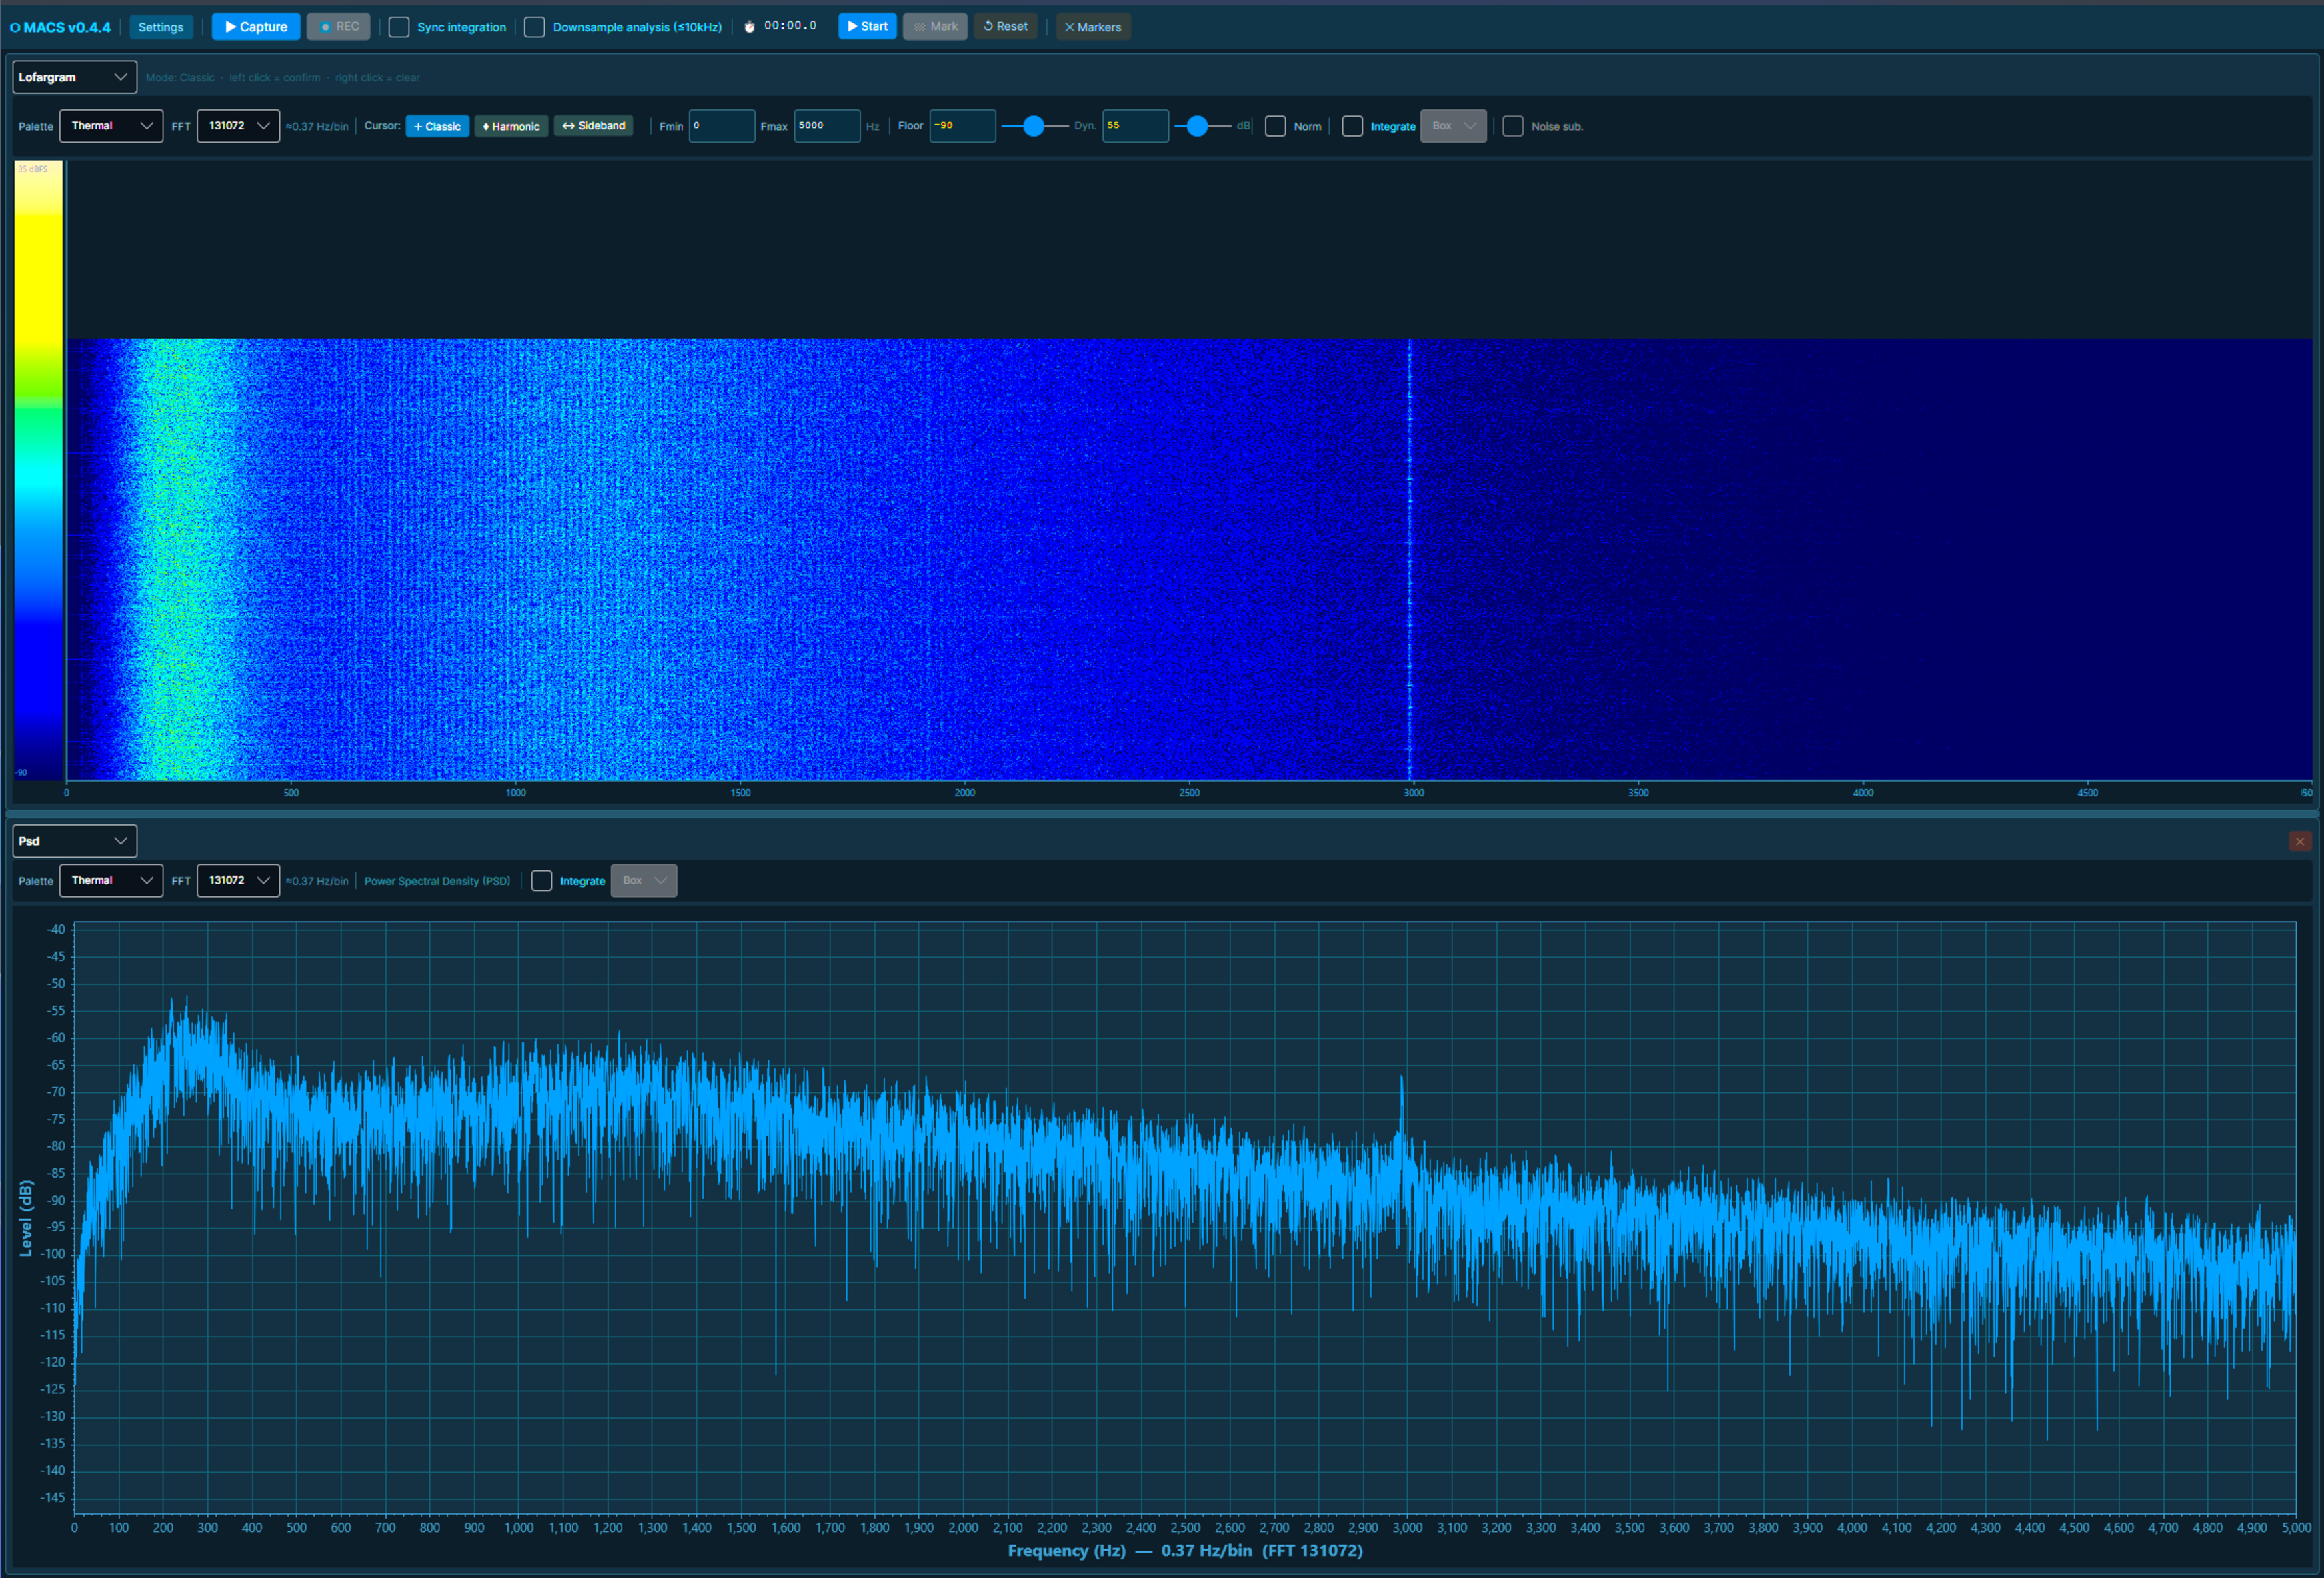
\includegraphics[width=300px]{../img/actuals/Type55_03.pdf}
	\caption{LOFARgram Fmin = 0 Hz - Fmax = 5000 Hz}
\end{figure}

The LOFARgram whilst much more detailed should be familiar. It shows and confirms our findings from the in game tools.

\begin{compactenum}
    \item Initial MNW narrowband screen shows a broad spectrum of noise between 150 Hz and 400 Hz.
    \item Another fainter band between 1050 Hz and 1350 Hz
    \item A high pitched whine / whistle at 3 kHz
    \item Narrow band does not have the distinctive lines associated with diesel firing
\end{compactenum}

\begin{figure}[ht]
	\centering
	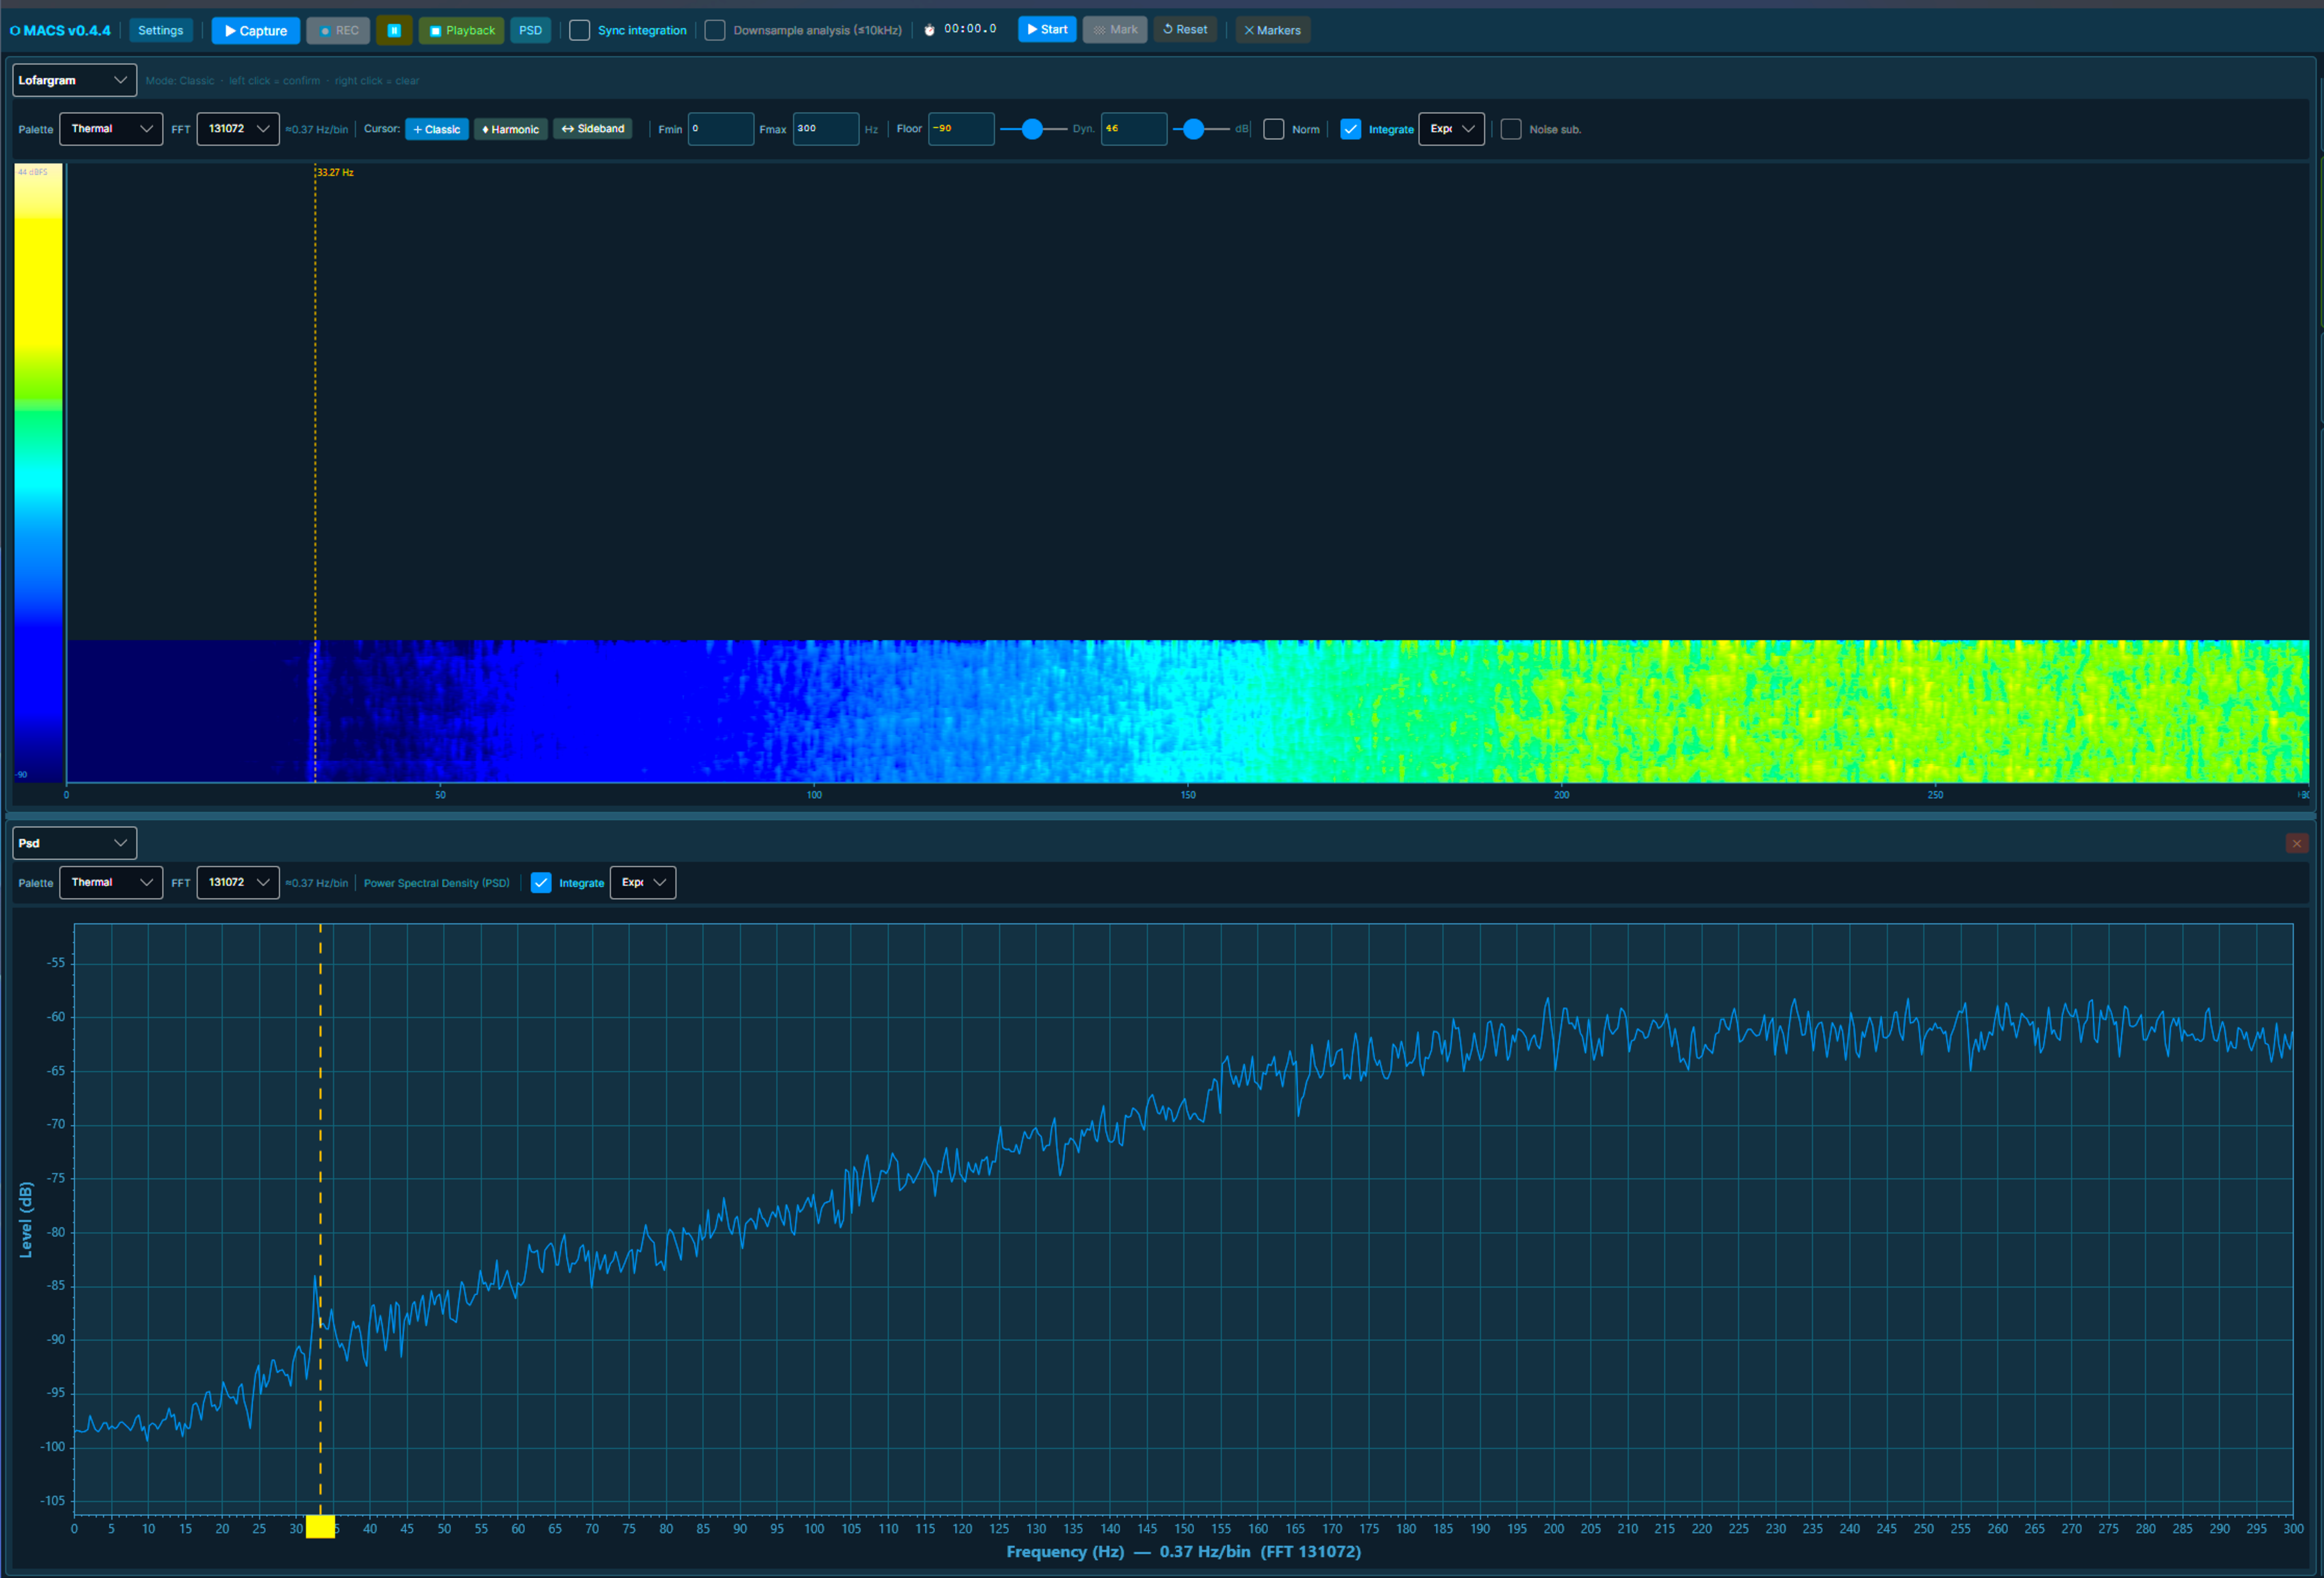
\includegraphics[width=300px]{../img/actuals/Type55_04.pdf}
	\caption{LOFARgram Fmin = 0 Hz - Fmax = 500 Hz}
\end{figure}

We repeat the plot but this time we reduce the Fmax parameter to 500 Hz because it would be useful to see if there are any fainter tonals that are crammed against the left hand side of the chart. Using the following settings we get Figure 20 revealing a hidden tonal which also confirms our earlier findings, the faint tonal seen in MNW is confirmed and narrowed down to 33.27 Hz

\begin{compactenum}
    \item Fmin = 0 Fmax = 500
    \item Floor = -90 Dyn 46
    \item Norm = Off
    \item FFT Overlap = Off
    \item FFT = 131072
    \item LOFARgram integration = Exp Box frame count = 16 Exponential time constant = 8 Fixed duration = 5
\end{compactenum}

The DEMON clearly shows a lone dual-sync tonal at 2.21 Hz Figure 21, which translates to 132.6 RPM closely matching audio SRPM. The line has a dual structure with a helical appearance which could possibly indicate a dual shaft.There is some indication of sidebands around the 2.21 Hz tonal which may indicate some modulation either by propellers or some other source.

\begin{figure}[H]
	\centering
	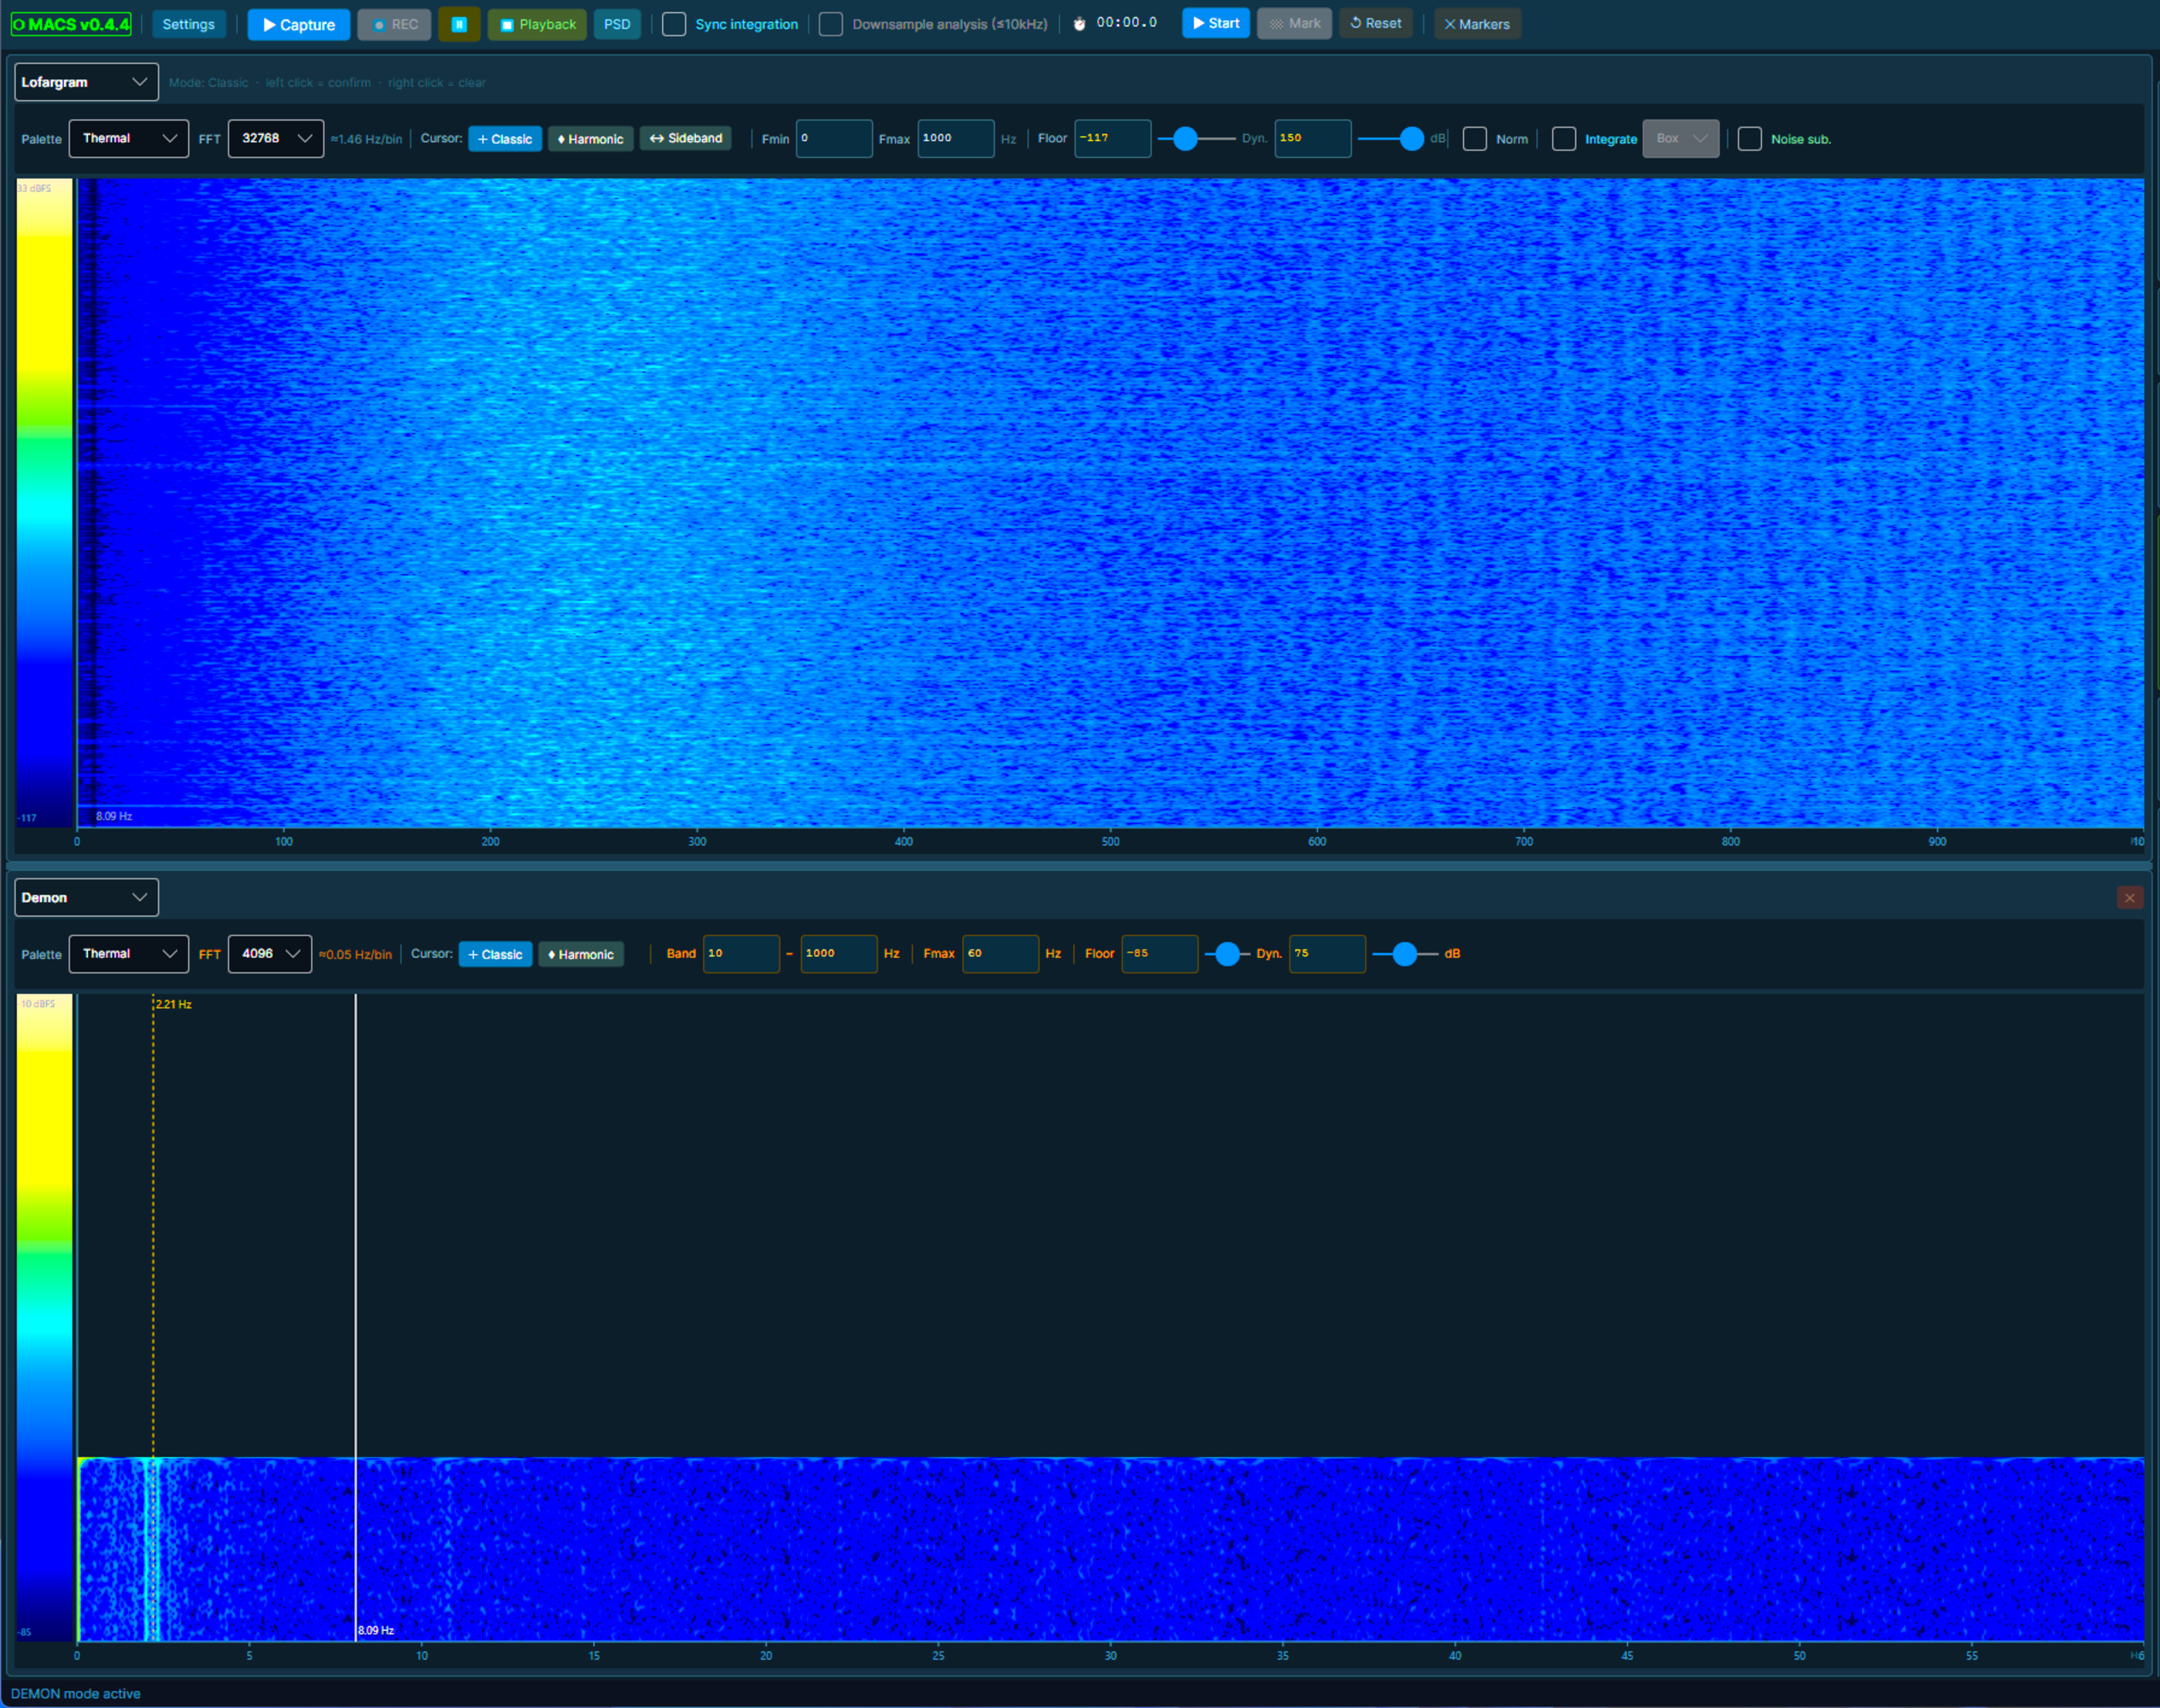
\includegraphics[width=300px]{../img/actuals/Type55_05.pdf}
	\caption{DEMON}
\end{figure}

There are also indications of higher tonals which fall very closely on the harmonics of the blade rate at 11 Hz. The third harmonic would be about 33 Hz and would be reinforced by the shaft harmonic. This is pure speculation but is a possible explanation for the faint line at 33 Hz.

\textbf{Classification}

We have enough information now to posit a classification for this vessel, which we will classify as potential warship, confirmed by spectral analysis.

\begin{compactenum}
    \item 5 blades with a high pitch turbine
    \item No diesel audio
    \item Broad noise bands
    \item Lack of sound usually associated with diesel engines
\end{compactenum}


Four ships in the recognition database match the noise band and 33 Hz signature

\begin{compactenum}
    \item Fuyu AOR: 22.3 kts at 134 RPM
    \item Ticonderoga CG: 24.2 kts at 134 RPM
    \item Renhai Type 055 DDG: 18.9 kts at 134 RPM
    \item Arleigh Burke DDG: 20 kts at 134 RPM
\end{compactenum}


Speed estimates are calculated from $SR \times (Max Speed \div Max RPM)$ (found from the recognition manual)

All three exhibit a very faint tonals around 30 - 34 Hz and a moderate noise band in the correct position.

For the Arleigh Burke the reported noise band and 30 Hz tonal are supposed to look much stronger. This questions this attribution suggesting medium confidence The Fuyu would be close to max speed (22 kts) at this SR which makes this a less likely candidate. Likewise a Ticonderoga would also be 10 kts below its maximum which would tend to suggest the diffuse noise band would be broader and more prominent.

\textbf{On the balance of probabilities the best fit based on the information we have is that our target is a Type 055 Renhai.}

\subsection{Illustrated Example 2: LOFAR - DEMON - Cepstrum}
\large Difficulty Rating \includegraphics{../img/actuals/Stars/"3 Stars.jpg"}

\begin{advisory}
    \textbf{Note: }Figures 22 - 27 were produced by the simulation engine not MACS. The equivalent MACS images are included in the download package.
\end{advisory}

This exercise demonstrates how a relatively complicated acoustic signal can be examined through three complementary forms of analysis: LOFAR, DEMON and cepstrum. Each technique approaches the signal differently. More importantly, the observations can be compared with one another and with the mathematical relationships expected from rotating machinery.

\textbf{Set Up:}
\begin{compactenum}
    \item Download and extract \texttt{"IE2 LOFAR DEMON Cepstrum.zip"}
    \item You should have the following directory structure.
    \begin{compactitem}
        \item csv
        \item img
        \item matlab
        \item python
        \item sound
    \end{compactitem}
    \item Using the matlab and python programs is discussed in Appendix D
\end{compactenum}

\textbf{Signal characteristics: }The supplied WAV has known parameters:
\begin{compactitem}
    \item Sample rate: 4,000 Hz
    \item Duration: 60 seconds
    \item Mean shaft rate: 1.30 Hz
    \item Shaft speed: 78 rpm
    \item Propeller blades: 5
    \item Blade rate: 6.50 Hz
    \item Second blade-rate harmonic: 13.00 Hz
    \item Machinery carriers: 150, 310, 620 and 900 Hz
    \item Additional machinery tonals: 48 and 96 Hz
\end{compactitem}

The relationship is: $\text{Shaft speed} = 60 \times 1.30 = 78\ \mathrm{rpm}$ and: $\text{Blade rate} = 5 \times 1.30 = 6.50\ \mathrm{Hz}$. A small ±0.025 Hz shaft-rate variation is included so the signal is not unrealistically perfect. Since we know what the two major fundamentals are the aim of the exercise is to see whether the three forms of analysis can recover them.

The synthetic example represents a five-bladed propeller turning at a Shaft Rate (SR) of 1.30 Hz, equivalent to 78 RPM. Its corresponding Blade Rate (BR) is therefore 6.50 Hz, with further related structure at multiples such as 13.00 Hz.

The objective is not simply to find those numbers in a graph. The exercise demonstrates the reasoning process by which several apparently different observations may be recognised as manifestations of the same underlying mechanical process.

\subsubsection{The Waveform}

The first image shows the acoustic waveform in the time domain.

\begin{figure}[h]
	\centering
	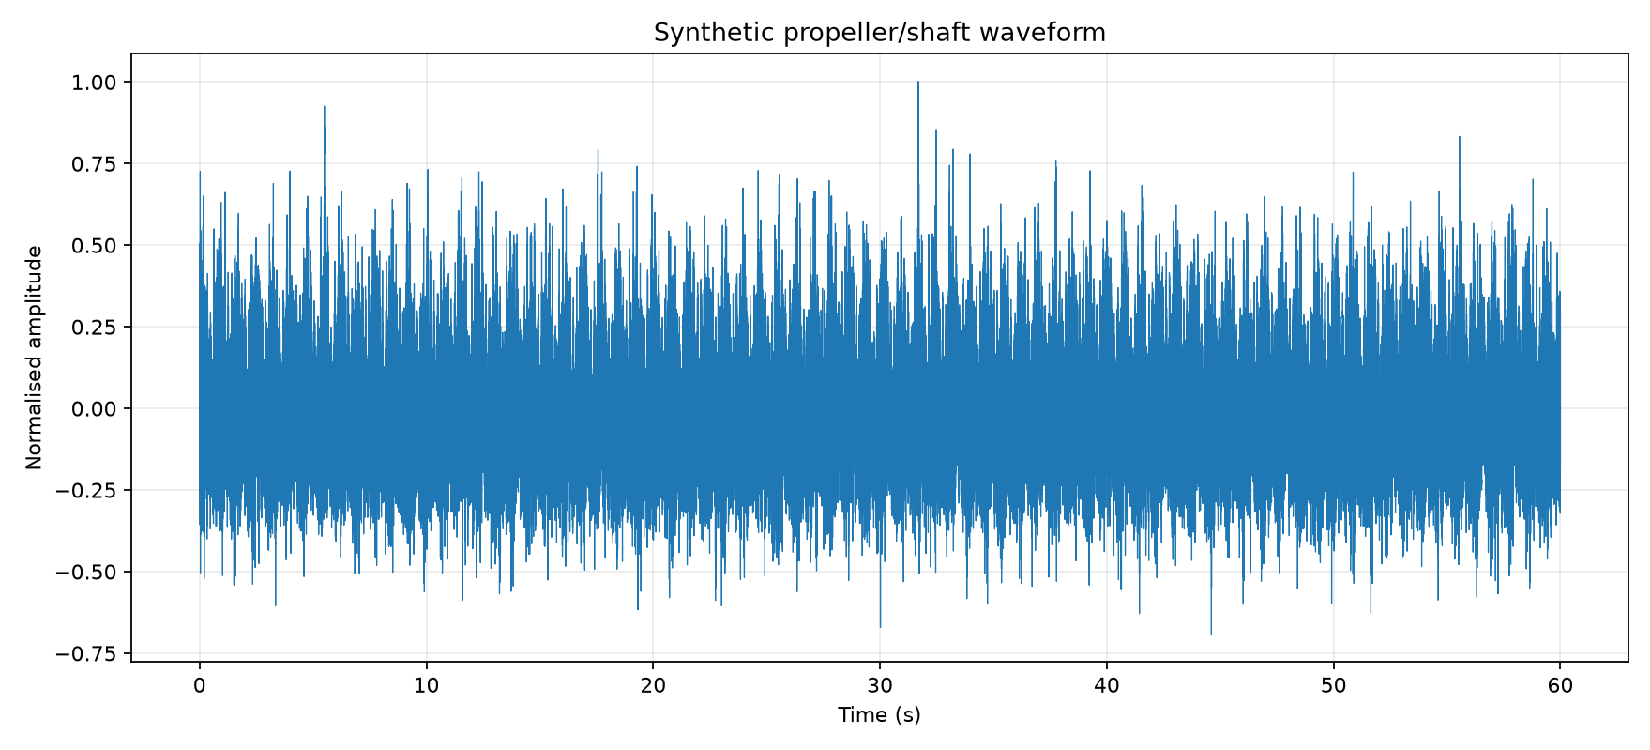
\includegraphics[width=350px]{../img/actuals/01_waveform.pdf}
	\caption{The Waveform}
\end{figure}

At this stage, the complete signal is represented as amplitude against time. Although the waveform confirms the presence and evolution of acoustic energy, most of the useful mechanical relationships are difficult to determine directly by eye. This is an important starting point. Information can be present in a signal without being visually obvious in the time waveform. The remaining analyses therefore transform or process the same underlying information to make particular characteristics easier to observe.

\subsubsection{The LOFAR Spectrogram}

The second image introduces frequency as a major analytical dimension.

\begin{figure}[h]
	\centering
	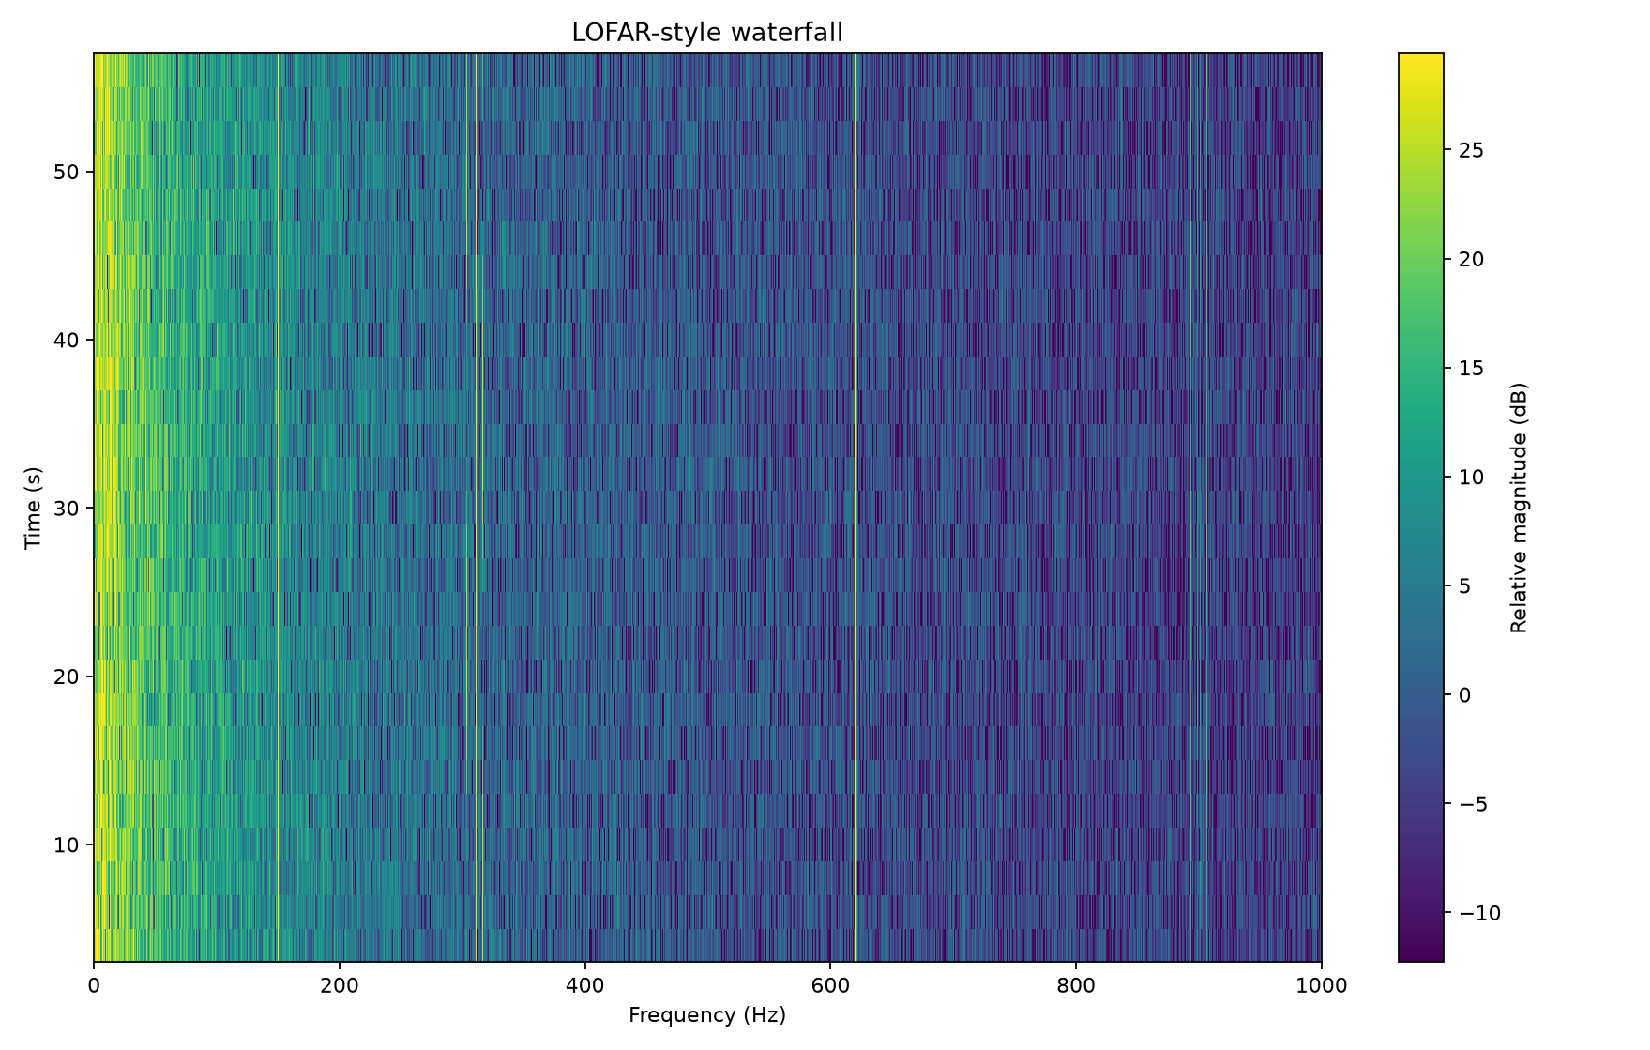
\includegraphics[width=350px]{../img/actuals/02_lofar_spectrogram.pdf}
	\caption{LOFAR Waterfall}
\end{figure}

The LOFAR-style display shows frequency against time, with intensity indicating the relative strength of spectral components. Persistent tonal components consequently appear differently from broadband energy or components that vary with time.

LOFAR asks: What frequency components are present, and how persistent are they?

This is the first move from observing a complex acoustic waveform towards identifying structure within it. The synthetic signal contains machinery-related frequencies and modulated carrier energy. LOFAR therefore provides evidence of the signal's spectral organisation. It can show tonals, harmonics and potentially the effects of modulation around stronger components. However, the presence of a frequency line does not by itself establish what produced it. The MACS review specifically identifies this distinction as important: a tonal peak is not automatically machinery. LOFAR therefore supplies the spectral evidence, but interpretation requires further corroboration.

\subsubsection{The Mean LOFAR Spectrum}

The third image collapses the time dimension by averaging the LOFAR spectra.

\begin{figure}[h]
	\centering
	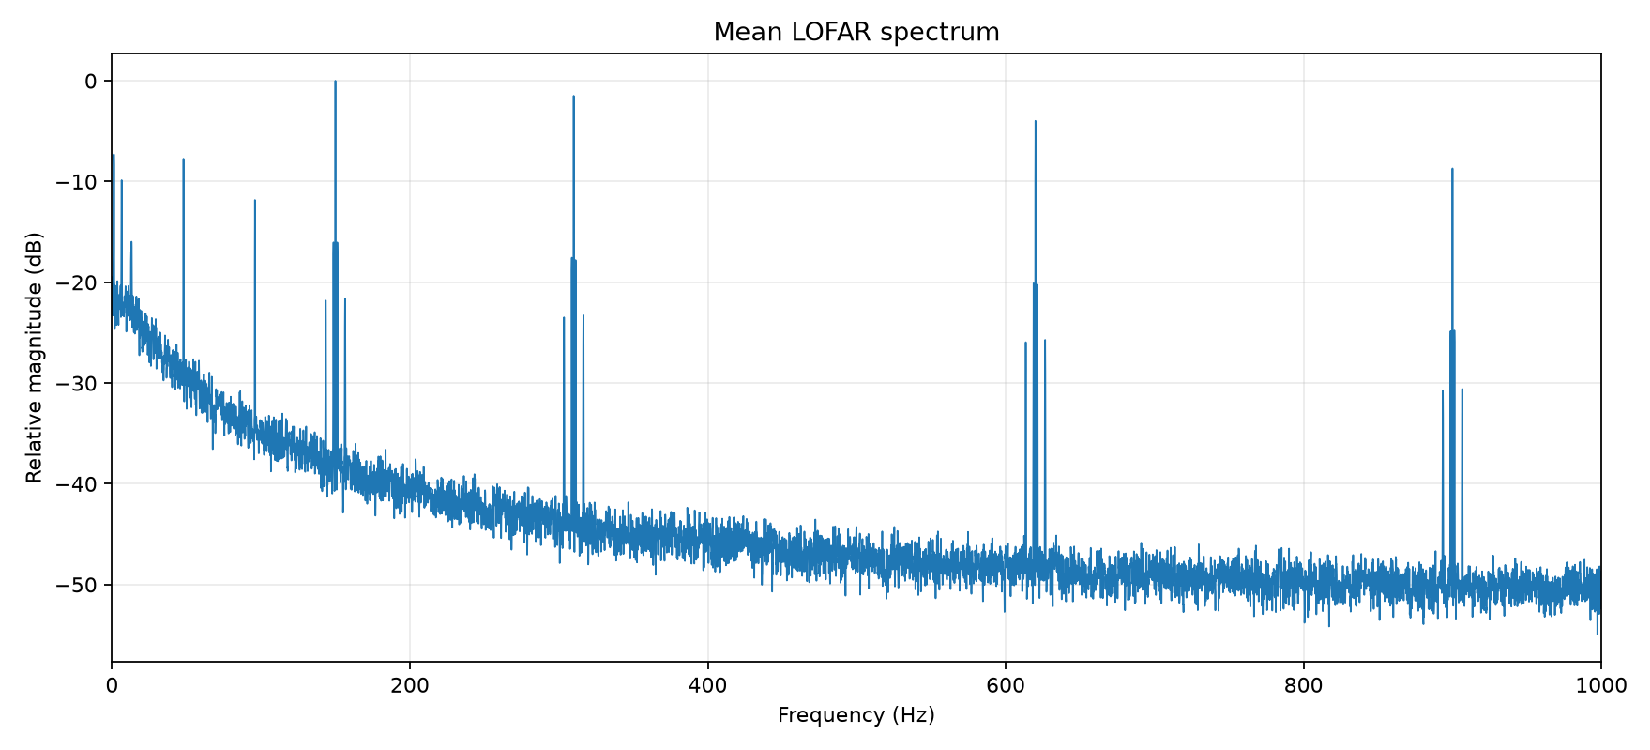
\includegraphics[width=350px]{../img/actuals/03_mean_lofar_spectrum.pdf}
	\caption{Mean LOFAR Spectrum}
\end{figure}

The result makes persistent frequencies easier to inspect quantitatively. The distinction between Images 2 and 3 is useful:

 \begin{compactitem}
    \item The LOFAR spectrogram answers when and where spectral energy occurs;
    \item The mean spectrum emphasises which spectral components persist strongly across the observation.
 \end{compactitem}


A peak in the mean spectrum is consequently an analytical clue rather than an automatic identification. Relationships between peaks matter considerably more. If components show harmonic spacing, sideband relationships or other regular structure, the analyst has a basis for asking whether they share a common mechanical origin.

This naturally leads to DEMON analysis.

\subsubsection{The DEMONgram}

DEMON provides a fundamentally different view of the signal.

\begin{figure}[h]
	\centering
	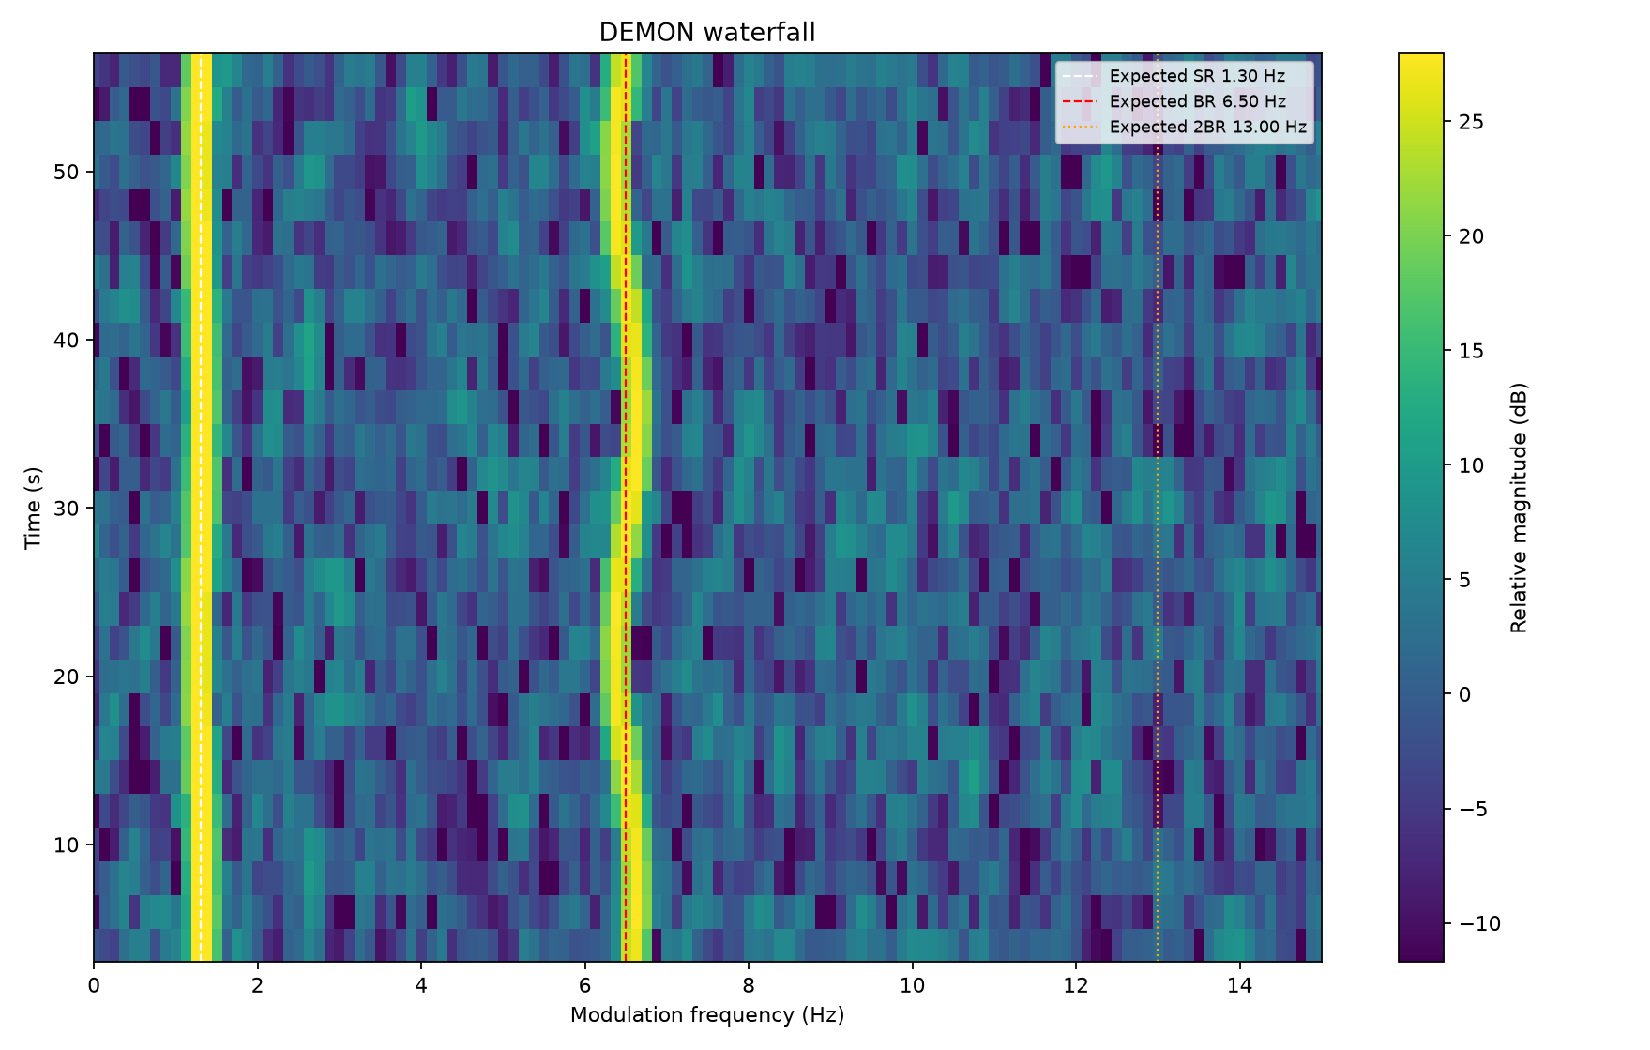
\includegraphics[width=350px]{../img/actuals/04_demongram.pdf}
	\caption{DEMON Waterfall}
\end{figure}

Rather than simply asking which acoustic frequencies are present, DEMON examines periodic amplitude modulation within a selected acoustic band. This distinction is fundamental and was specifically highlighted as a strength in the review of the MACS material: DEMON extracts modulation frequencies, which are subsequently interpreted through shaft and blade relationships.

The DEMONgram therefore asks: At what rates is the acoustic energy being modulated, and how do those rates behave with time?

That question is particularly relevant to rotating machinery.

In the synthetic example there is a known Shaft Rate:

$SR=1.30\text{ Hz}$

and a five-bladed propeller.

The corresponding Blade Rate is therefore:

$BR=B\times SR$

where BB is the number of blades.

Thus:

$BR=5\times1.30=6.50\text{ Hz}$

The DEMON display allows those low-frequency modulation relationships to become much more apparent than they may have been in the original waveform or conventional spectral display.

\subsubsection{The Mean DEMON Spectrum}

The fifth image is particularly useful for interpretation because it converts the DEMONgram into an averaged modulation spectrum. The principal frequencies of interest are:

$1.30\text{ Hz},\quad6.50\text{ Hz},\quad13.00\text{ Hz}$

These are not three arbitrary numbers, they form a mathematically related family.
\begin{figure}[h]
	\centering
	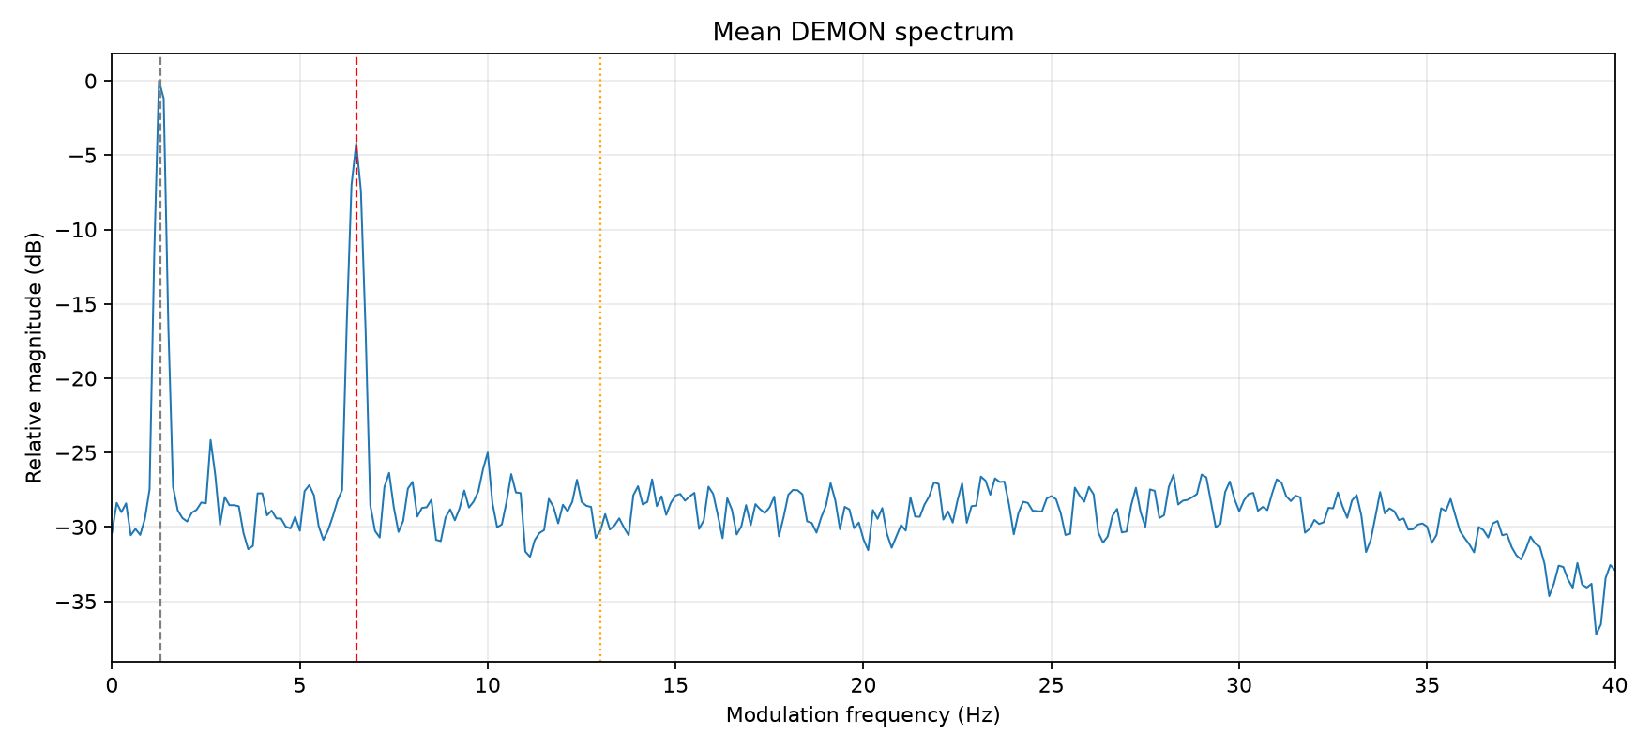
\includegraphics[width=350px]{../img/actuals/05_mean_demon_spectrum.pdf}
	\caption{Mean DEMON spectrum}
\end{figure}

\begin{advisory}
\textbf{Why the 13 Hz line is unclear: }The second Blade Rate harmonic is not convincingly visible in the supplied DEMONgram. That is a limitation of the synthetic signal rather than something that should be explained away in the guide.
\end{advisory}

The 1.30 Hz component corresponds to the known Shaft Rate, while:

$\frac{6.50}{1.30}=5$

This is consistent with a five-bladed propeller.

Furthermore:

$13.00=2\times6.50$

so 13.00 Hz is consistent with the second harmonic of Blade Rate.

The value of the DEMON spectrum therefore lies not merely in finding a strong peak, but in recognising a coherent pattern:

$SR\rightarrow BR\rightarrow2BR$

That provides substantially more meaningful evidence than interpreting any one component alone.

\subsubsection{The Real Cepstrum}

The sixth image examines the signal from yet another perspective.

\begin{figure}[h]
	\centering
	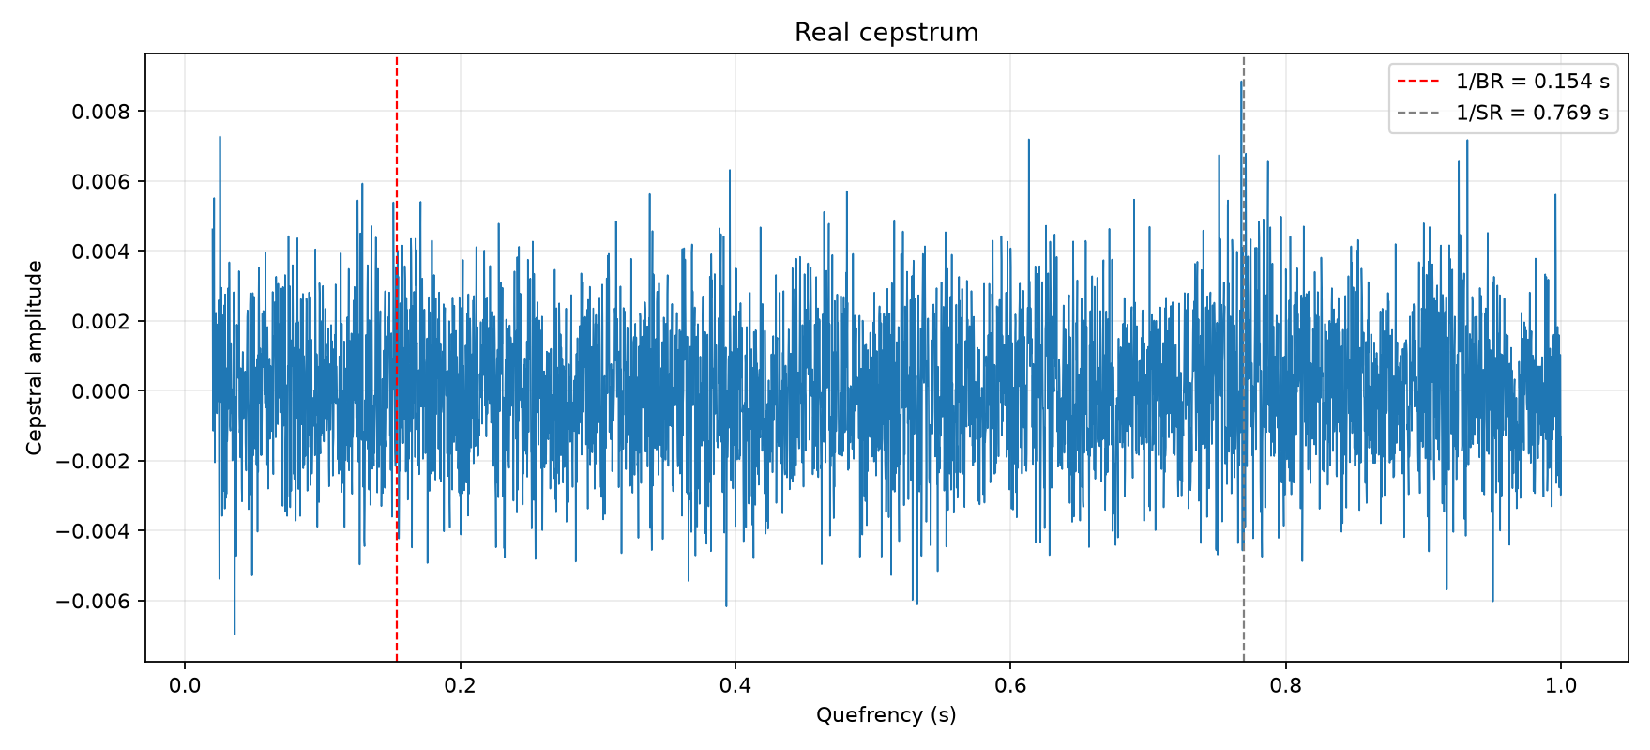
\includegraphics[width=350px]{../img/actuals/06_real_cepstrum.pdf}
	\caption{Real Cepstrum}
\end{figure}


Cepstral analysis is useful for revealing regular spectral spacing. Its horizontal coordinate is termed quefrency and has units of time.

The basic relationship is:

\[
    q=\frac{1}{\Delta f}
\]

where $\Delta f$ is a repeating frequency spacing.

For the 6.50 Hz Blade Rate relationship:

\[
    q=\frac{1}{6.50}\approx0.154\text{ s}
\]

For the 1.30 Hz shaft relationship:

\[
    q=\frac{1}{1.30}\approx0.769\text{ s}
\]

The significance of the cepstrum is therefore that it provides another way of searching for periodic organisation within the signal.

The real cepstrum contains numerous peaks because it responds to regular spacing anywhere in the acoustic spectrum. The vertical markers at 0.154 s and 0.769 s are expected quefrencies calculated from the Blade Rate and Shaft Rate estimated by DEMON. They are reference positions, not automatic detections. A peak at either position supports the interpretation only when it is locally prominent and agrees with independent LOFAR and DEMON evidence.

\begin{learnpoint}
    \textbf{Learning Point} \\
    You should be cautious in identifying 0.154 s and 0.769 s as BR and SR from this cepstrum alone. First obtain candidate rates from DEMON and supporting spectral structure from LOFAR, then uses the cepstrum to look for compatible periodic spacing. If the expected positions do not stand out locally, the cepstrum has not added strong corroborating evidence in that particular recording.
\end{learnpoint}


To summarise so far:

\begin{compactitem}
    \item \textbf{LOFAR} presents spectral structure.
    \item \textbf{DEMON} presents modulation structure.
    \item \textbf{CEPSTRUM} presents periodic spectral-spacing structure.
\end{compactitem}

When compatible relationships appear in these different representations, confidence in the interpretation can increase.

\begin{learnpoint}
    \textbf{Learning Point}\\
    No individual display needs to carry the whole interpretation. LOFAR may reveal persistent spectral features but leave their origin uncertain. DEMON may expose a family of modulation rates. The cepstrum may independently indicate corresponding periodic spacing. Mathematical relationships can then test whether these observations form a physically coherent pattern. This layered confirmation principle is the means by which an analyst avoids over-interpreting one attractive spectral peak.
\end{learnpoint}
\subsubsection{Correlating the Evidence}

This is the central purpose of the exercise.

The analytical progression can be thought of as:

\begin{figure}[h]
	\centering
	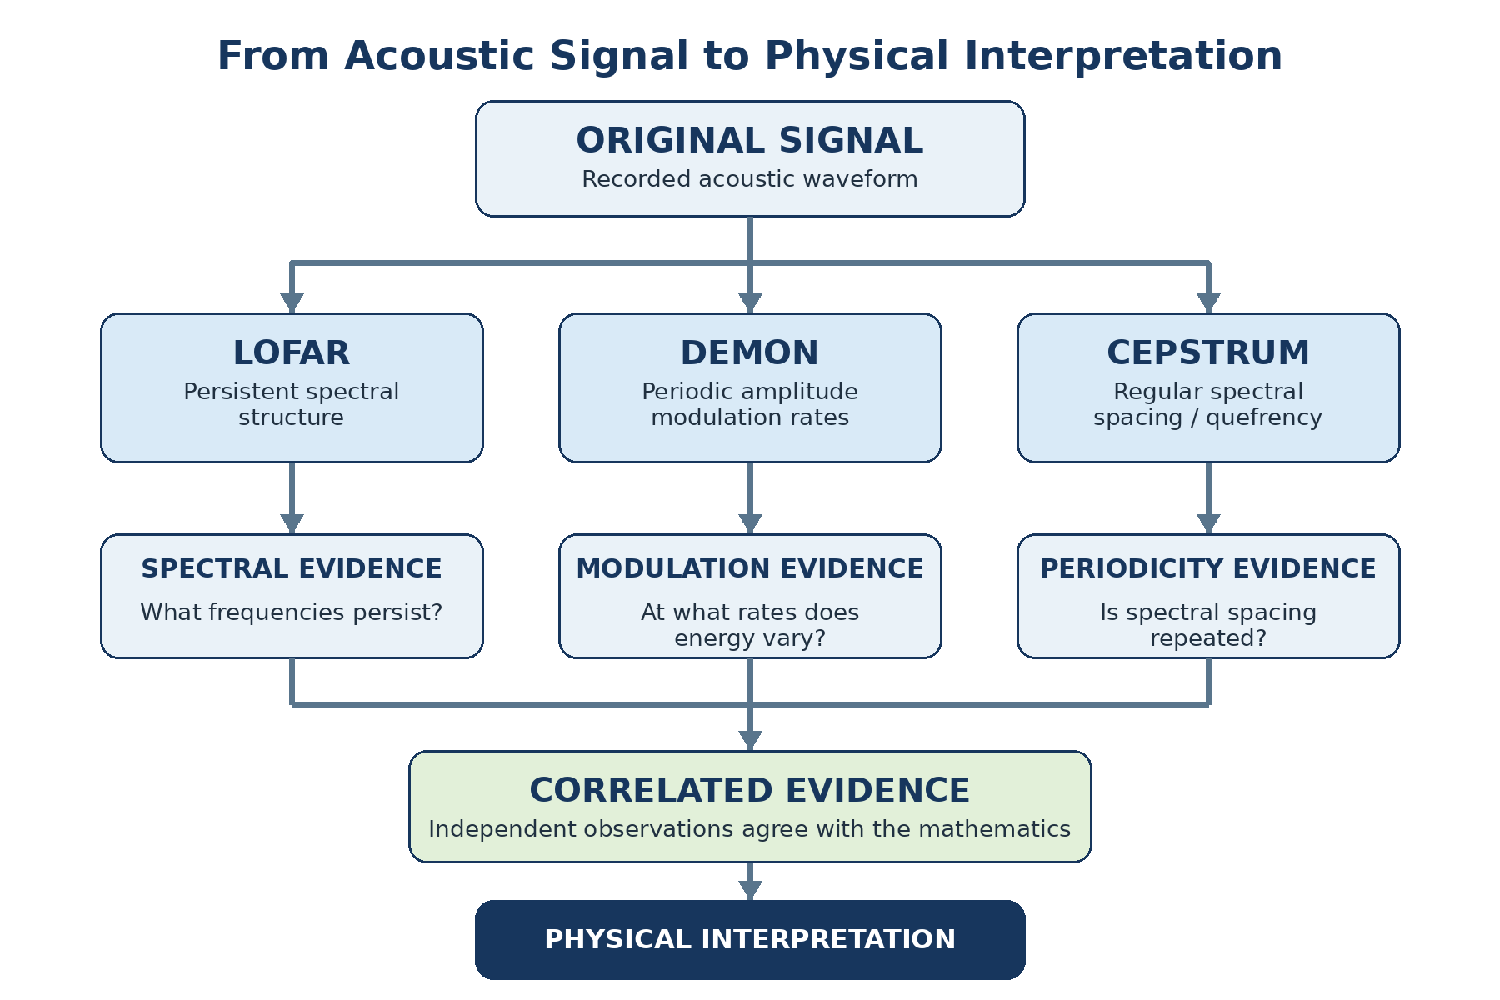
\includegraphics[width=350px]{../img/actuals/LDC_evidence_flow.pdf}
	\caption{LOFAR, DEMON, CEPSTRUM evidence flow}
\end{figure}



\subsubsection{Summary of Findings}

The synthetic example begins with a known:
\[
    \boxed{SR=1.30\text{ Hz}}
\]

Shaft frequency converts directly to rotational speed: $RPM=60\times SR$

therefore:
\begin{align*}
    RPM &= 60\times1.30 \\
    RPM &= \boxed{78 RPM}
\end{align*}

For five propeller blades: $BR=B\times SR$ and therefore:
\begin{align*}
    BR = 5\times1.30 \\
    \boxed{BR = 6.50\text{ Hz}}
\end{align*}

The next Blade Rate harmonic occurs at:
\begin{align*}
    BR = 2\times6.50 \\
    \boxed{BR = 13.00\text{ Hz}}
\end{align*}
    
Conversely, if SR and BR were measured without knowing the blade count:
\begin{align*}
    B &= \frac{BR}{SR} \\[1ex]
    B &= \frac{6.50}{1.30} \\[1ex]
    B &= \boxed{5}
\end{align*}

Finally, the corresponding reciprocal relationships provide expected cepstral quefrencies:
\[
    q_{BR}=\frac{1}{6.50}\approx\boxed{0.154\text{ s}}
\]

and:
\[
    q_{SR}=\frac{1}{1.30}\approx\boxed{0.769\text{ s}}
\]

The exercise therefore brings the analysis full circle. LOFAR identifies spectral structure, DEMON exposes modulation structure, and the cepstrum searches for periodic spectral spacing. The mathematical relationships between Shaft Rate, rotational speed, Blade Rate, harmonics and quefrency then provide a common framework within which those observations can be compared.

The important finding is consequently not simply “there is a peak at 6.5 Hz”. It is the much stronger chain of reasoning:
\[
    \boxed{ 1.30\text{ Hz} \rightarrow 78\text{ RPM} \rightarrow 5\times1.30 \rightarrow 6.50\text{ Hz} \rightarrow 2\times6.50 \rightarrow 13.00\text{ Hz} }
\]

supported by complementary views of the same underlying signal.

\begin{learnpoint}
    \textbf{Learning Point:}\\
    This exercise demonstrates that acoustic analysis becomes most persuasive when observations from different analytical domains agree with one another and with the underlying mathematics, rather than when an interpretation depends upon a single conspicuous peak. This reflects the broader principle that the evidence should support the hypothesis. That fits with the MACS Guide's broader analytical approach: LOFAR asks what spectral structure exists, DEMON reveals modulation behaviour, and the cepstrum looks for compatible periodic spacing. The interpretation becomes more concrete when those independent observations agree with the underlying physics and mathematics
\end{learnpoint}

\subsection{Exercise 1: Finding the way}
\textcolor{commentGreen}{*** WIP ***}

This exercise is to help you find your way around MACS, identify fundamental tonals and to optimize settings.

\subsection{Exercise 2: Sabre Dance}
\begin{compactenum}
    \item Download and extract \texttt{"Sabre Dance".zip}
    \item Carefully read the exercise \texttt{Outline.pdf} and then follow the instructions
\end{compactenum}

\subsection{Exercise 3: Snaky Medusa}
\textcolor{commentGreen}{*** WIP ***}
\begin{compactenum}
    \item Download and extract \texttt{"Snaky Medusa".zip}
    \item Carefully read the exercise \texttt{Outline.pdf} and then follow the instructions
\end{compactenum}

\subsection{Exercise 4: Classification \#1}
\begin{compactenum}
    \item Download and extract \texttt{"EX4 Classification 1".zip}
    \item Carefully read the exercise \texttt{Outline.pdf} and then follow the instructions
\end{compactenum}

\subsection{Exercise 5: Classification \#2}
\begin{compactenum}
    \item Download and extract \texttt{"EX5 Classification 2".zip}
    \item Carefully read the exercise \texttt{Outline.pdf} and then follow the instructions
\end{compactenum}

\subsection{Final Test}
\begin{compactenum}
    \item Download and extract \texttt{"Exam Distribution".zip}
    \item Carefully read the exercise \texttt{Exam Outline.pdf} and then follow the instructions
\end{compactenum}

\pagebreak
